\chapter{Multi-Objective Bilevel Optimization}


\begin{tcolorbox}
\textit{The work presented in this chapter has been published in the following article:}
\small
\begin{itemize}
\item \textbf{{Islam,~M.~M.}}, {Singh, H.K.} and {Ray, T.}, ``A nested differential evolution based algorithm for solving multi-objective bilevel optimization problems,'' in {\em Proceedings of the Australasian Conference on Artificial Life and Computational Intelligence (ACALCI)}, Canberra, Australia, vol. 9592 of {\em Lecture Notes in Artificial Intelligence}, pp. 101--112, Springer, 2016.
\end{itemize}
\end{tcolorbox}

\section{Background}
\label{sec:intro}

Multiple criteria decision making~(MCDM) is an established field which deals with search for optimum solutions and selection of solutions from the Pareto optimal set for problems involving more than one conflicting {\color{blue}objectives}. The two aspects of MCDM, \emph{search for solutions} and \emph{selection of solutions} are formally termed as multi-objective decision making~(MODM) and multi-attribute decision making~(MADM) respectively~\cite{yang1994evidential}. The latter involves choosing a solution by a decision maker~(DM) from a given set of Pareto optimal solutions, and is the focus of this study. MADM methods capture preferences of the DM via inter-attribute/criteria comparisons and use them to identify the most preferred solution(s) from the given set. In the context of \textcolor{blue}{multi-objective} optimization involving computationally expensive simulations or lengthy physical experiments, it may be \textcolor{blue}{viable to search for and present only a small number of solutions that are (or are close to) Pareto optimal in the outcome space to the DM. Using these outcomes, one can assess the limits of performance~(minimum and maximum values) in terms of each objective. However, the inherent sparsity of the given Pareto optimal outcomes in a high-dimensional objective space poses severe challenges to the effectiveness of decision making}~\cite{ruzika2005approximation}. The method introduced in this paper attempts to generate interpolated outcomes from the given set of Pareto optimal outcomes, \textcolor{blue}{in order to offer} additional choices~({\color{blue}albeit approximated}) for more informed decision making.

The problem is referred to in the literature as Pareto front interpolation and an excellent review of the methods along with a detailed classification appears in~\cite{ruzika2005approximation}. Discussion on various recent forms of Pareto interpolation appear in ~\cite{hartikainen2011constructing}. The methods can be classified broadly into: 

\begin{itemize} 
	\item Methods that rely on visualization to identify preferred point(s)~\cite{monz2008pareto,lotov2008visualizing}. Other similar approaches include constructing convex hulls enclosing infeasible solutions~\cite{missoum2007convex} or constructing polynomial response surface approximations {\color{blue}where one objective is expressed as a function of other objectives~\cite{goel2007response}},  
	\item Methods that are only applicable to convex fronts such as those introduced in \cite{monz2006pareto,eskelinen2010pareto} and the enumeration and approximation error guided sandwich method introduced in~\cite{bokrantzdual},
	\item {\color{blue} Methods that rely on global convergence to obtain a strict superset of Pareto optimal solutions~\cite{lovison11singular,lovison2013mo,lovison2015lip}}.
	\item Methods that are only applicable to non-convex fronts~\cite{berezkin2006hybrid}. 
	\item {\color{blue}Methods that are applicable to both convex and non-convex fronts~\cite{hartikainen2010computationally,hartikainen2012paint,hartikainen2011demonstrating,hartikainen2014paint,martin2005approximating,hillermeier2001homo,hillermeier2001nmo,wiecek2016mo,kuhn2016box}}.
\end{itemize}

{\color{blue}
	Since our focus is on development of algorithms that are applicable across both convex, non-convex, mixed and potentially degenerate fronts, we discuss the last class of methods in greater details. The approach introduced by Hartikainen~\cite{hartikainen2012paint,hartikainen2014paint} is referred to in literature as PAINT~(PAreto INTerpolation) and it offers the decision maker a set of piecewise linearly interpolated outcomes in the form of a collection of \emph{inherently non-dominated} simplexes. 
	
	In order to construct the approximation using $N$ given Pareto outcomes in $M$ dimensions, PAINT starts by generating a set of candidate simplexes, and uses certain rules to eliminate undesirable ones. The remaining set of simplexes form the final approximation. A \emph{simplex} (in $\mathbb{R}^n$) is a special case of a convex polytope, namely one with exactly $n+1$ extremal points (the convex hull of $n+1$ points in general position, that is to say they do not lie in a $n-1$ dimensional affine subspace). Throughout this paper, the term $n-$simplex will be used to denote a simplex with $n+1$ vertices, a convention consistent with earlier works~(e.g.\cite{hartikainen2012paint}) in the area.
	
	The initial set of simplexes is generated through \textit{Delaunay triangulation}, which is a concept widely used in computational geometry for reconstruction of surfaces. For $M$-dimensional points, Delaunay Triangulation creates a set of polyhedrons with $(M+1)$ vertices~(e.g. tetrahedron for a 3-objective problem), which are thus $M$-simplexes. Each of these simplexes are then further successively broken down into simplexes of lower degree~(e.g. tetrahedron~(3-simplex) is divided into the constituting faces~(2-simplexes), which are in turn divided into the constituting edges~(1-simplexes), and so on). The resulting set of \{$M,(M-1),(M-2) \ldots 0$\}$-$simplexes form the initial candidate simplex set. The given Pareto optimal outcomes are also part of this set, and are 0-simplexes. 
	
	From the initial set, certain simplexes are eliminated using these rules\footnote{In \cite{hartikainen2012paint}, the first two rules are covered as a single rule R1, but we differentiate them as R1.1 and R1.2}: (R1.1) \emph{point-simplex dominance}, i.e., a given Pareto outcome dominates or is dominated by a simplex, (R1.2)\textit{self dominance}, i.e., an point in a simplex dominates another, and (R2) \textit{simplex-simplex dominance} a point on one simplex dominates a point on another simplex. {\color{blue}In order to perform these domination comparisons between any two simplexes~(or between a given outcome and a simplex), a linear programming problem~(LP) is formulated and solved~\cite{hartikainen2012paint}}. These eliminations are performed in a particular sequence, and all the simplexes which are not eliminated by the above rules form the final approximation.  
	
	PAINT delivers an \textit{inherently non-dominated} approximation, which means that none of the interpolated outcomes could dominate or be dominated by the given outcomes as well as each other. Additionally, the set is also \textit{maximal}, which implies that no other simplex could be added in the final set without violating inherent non-dominance.} The concept of inherent non-dominance is demonstrated to be a useful property in the approximation set as it avoids {\color{blue}dominated/dominating} outcomes that can mislead a decision maker. This is in contrast with the other approaches that may generate outcomes that dominate~(or are dominated by) the existing Pareto outcomes.

{\color{blue}
	While PAINT delivers a suitable approximation in its own right, in this study, we offer a different perspective on constructing such approximations, which could further enhance the interpolated outcomes delivered. The key premise we present is that enforcement of inherent non-dominance could lead to loss of certain simplexes that could have been otherwise useful for decision making. These are the simplexes that are non-dominated with respect to all given Pareto outcomes but may dominate/be dominated by other \emph{interpolated} outcome(s). We refer to them as ``valid'' simplexes, and in our opinion, they should not be eliminated, but instead should be used to construct a more \emph{comprehensive} approximation. To explain the underlying context, we present two scenarios below.
}
\subsection{Possibility of achieving only one~(of many) interpolations} Consider the well known 3-objective DTLZ2 problem~\cite{deb2002scalable}. Let us assume that four Pareto optimal outcomes are provided to the DM, listed in Table~\ref{probstatdtlzvalid}. The Pareto optimal outcomes are presented in Figure~\ref{fig:dtlz2_valid}. Relying on a linear interpolation model, one can construct four possible triangular faces using these points and we refer them as the inner pair depicted in Figure~\ref{fig:dtlz2_inner1} and the outer pair depicted in Figure~\ref{fig:dtlz2_outer1}. It is important to take note that both outer and inner pairs are valid faces for interpolation, as points on the triangular faces are non-dominated with respect to the given set of Pareto optimal outcomes. PAINT by virtue of its Delaunay triangulation and elimination rules allows for the existence of only the outer pair thereby offering inherently non-dominated set of interpolated outcomes. {\color{blue}Note that the inherently non-dominated set delivered is \textit{not unique}, as one can be constructed using either pair.} 

{\color{blue}
	Secondly, the use of Delaunay Triangulation in PAINT inherently prevents construction of certain simplexes in the first place. The choice of using Delaunay Triangulation is predominantly driven by its geometric advantages in triangulating a surface, and not by dominance relationships among the given points as such. Therefore, there may exist simplexes that are \textit{not} generated as part of the initial set~(via method discussed above), but are non-dominated with respect to all given Pareto outcomes. Such simplexes are again ``valid'' and should not be excluded by default.}

\begin{table}[!ht]\scriptsize
	\centering
	\caption{Pareto outcomes and valid faces for DTLZ2}
	\label{probstatdtlzvalid}
	\tabcolsep=0.11cm
	\begin{tabular}{llll}
		\specialrule{.1em}{.1em}{.1em} 
		{\bf Point} & {\bf $F_1$} & {\bf $F_2$} & {\bf $F_3$} \\ \hline
		v1          & 0.9045    & 0.3015    & 0.3015    \\ \hline
		v2          & 0.6667    & 0.3333    & 0.6667    \\ \hline
		v3          & 0.3333    & 0.6667    & 0.6667    \\ \hline
		v4          & 0.6667    & 0.6667    & 0.3333    \\ 
		\specialrule{.1em}{.1em}{.1em}
	\end{tabular}
\end{table}

\begin{figure}[!ht]
	\centering
	\subfigure[Valid inner face pair for DTLZ2]{\label{fig:dtlz2_inner1}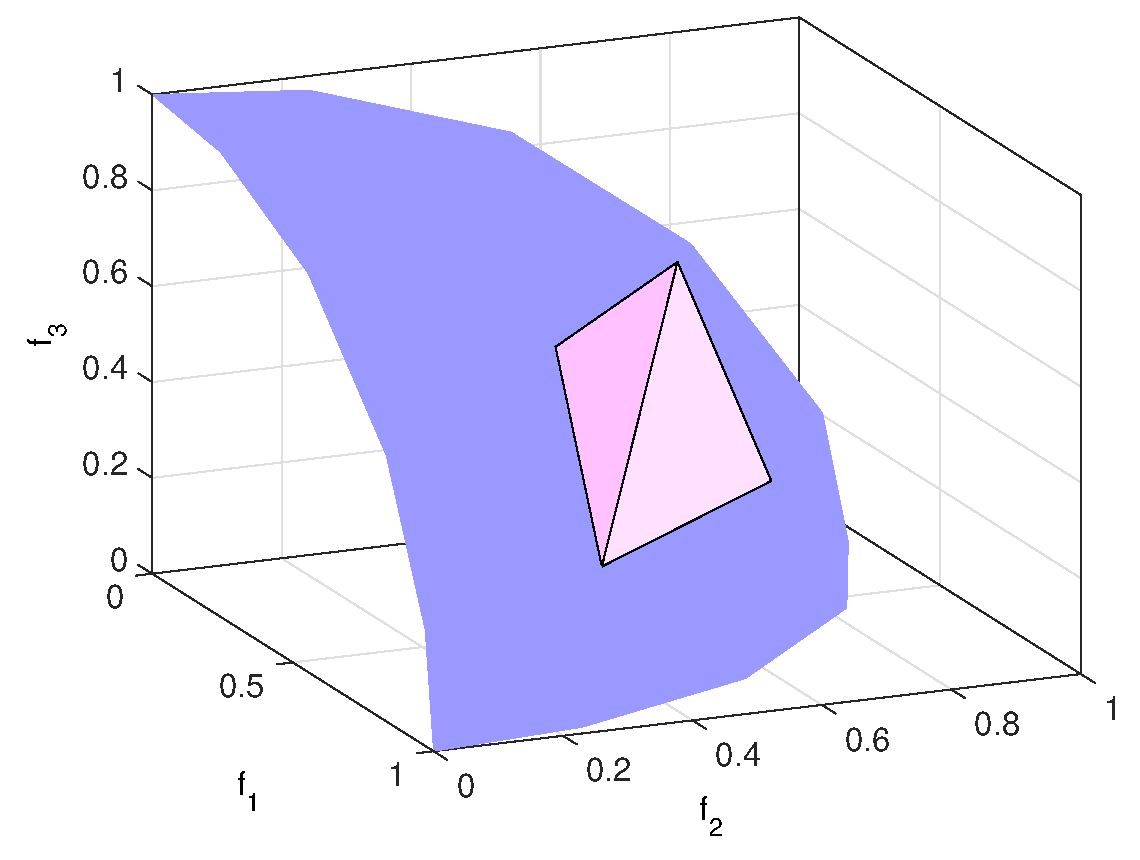
\includegraphics[width=0.40\linewidth]{dtlz2_inner1.eps}}
	\subfigure[Valid outer face pair for DTLZ2]{\label{fig:dtlz2_outer1}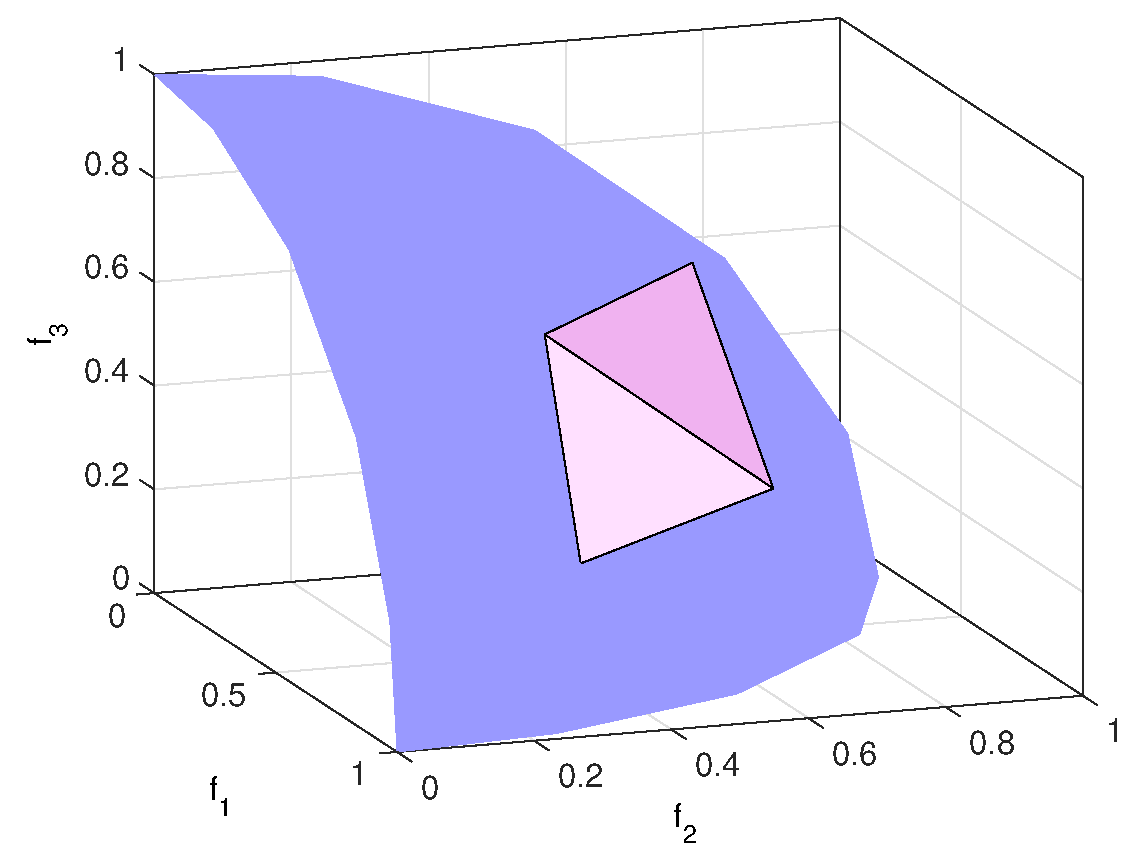
\includegraphics[width=0.40\linewidth]{dtlz2_outer1.eps}}
	\caption{Valid faces for DTLZ2}
	\label{fig:dtlz2_valid}
\end{figure}

\subsection{Possibility of missing on certain useful regions leading to discontinuities}

{\color{blue} We further highlight that imposing a condition of all simplexes being non-dominated to each other may lead to loss of certain valid simplexes, introducing undesirable \textit{discontinuities} in the final set delivered. As an illustration, consider the heat exchanger design example reported in \cite{hartikainen2010computationally}. One can observe a missing region~(one or more faces) in  Figure~\ref{fig:heat_exchanger_paint}, obtained using PAINT due to imposition of inherent dominance through rules R1 and R2 discussed earlier. Note that this elimination could be because of an \textit{interpolated outcome} dominating another \textit{interpolated outcome}, none of which are guaranteed to be Pareto optimal. Existence of a void in the approximation might dissuade a DM to look for a solution in that region. However, as depicted in Figure~\ref{fig:heat_exchanger_pli}, there exist simplexes which are non-dominated with respect to the given set of Pareto optimal outcomes. Given this characteristic, they should be treated as a valid choice for generating interpolated points for consideration of a decision maker.}


\begin{figure}[!ht]
	\centering
	\subfigure[Interpolation obtained from PAINT for heat exchanger problem]{\label{fig:heat_exchanger_paint}\includegraphics[width=0.40\linewidth]{heat_exchanger_paint.eps}}
	\subfigure[Interpolation obtained from proposed Pareto linear interpolation for heat exchanger problem]{\label{fig:heat_exchanger_pli}\includegraphics[width=0.40\linewidth]{heat_exchanger_approx_pli.eps}}
	\caption{Difference in the interpolations for Heat exchanger problem, with and without inherent dominance}
	\label{fig:dtlz2_paint_pli}
\end{figure}

The discussions presented above underpin the motivation for the proposed study. The main contributions of the study could be summarized as follows. 

\begin{enumerate}
	
	\item The proposed approach attempts to generate a \textit{comprehensive} set of possible interpolations which are non-dominated with respect to the given Pareto outcomes. Therefore, it does not use \textcolor{blue}{the} Delaunay triangulation to generate \textcolor{blue}{the} initial simplicial complex set. Instead it constructs all possible unique \textcolor{blue}{simplexes} with number of vertices $M$, $M-1$, through to 1, where $M$ is the number of objectives of the problem. Thus, given a set of Pareto optimal outcomes $PF$, such that $|PF|=N$,  there are $N\choose 1$ \textcolor{blue}{$0$-simplexes}, $N\choose 2$ \textcolor{blue}{$1$-simplexes}, $N\choose 3$ \textcolor{blue}{$2$-simplexes}, $\ldots$ $N\choose {M+1}$ \textcolor{blue}{$M$-simplexes}.  If any point within a \textcolor{blue}{simplex} dominates or is dominated by any point of $PF$, the \textcolor{blue}{simplex} is eliminated. However, as discussed above, it is possible that an interpolated outcome on one \textcolor{blue}{simplex} may dominate another interpolated outcome on a different \textcolor{blue}{simplex}. \textcolor{blue}{In this case the simplex will not be discarded}. 
	
	\item We highlight that the approach is amenable to parallelization, since the sequence of comparison in the approach outlined above has no impact on the final approximation obtained. 
	
	\item Furthermore, to offer a well distributed set of interpolated outcomes for decision making, a set of uniformly distributed weight vectors~(uniformly distributed along the hyperplane) are then constructed using systematic sampling. \textcolor{blue}{The} interpolated outcome(s) on the \textcolor{blue}{simplexes} along these directions are identified by solving a linear programming~(LP) problem, and these points are then added to the decision making set. Unlike previous approach(es), more than one solution can be delivered along a given direction~(for example, a point at both inner and outer face in the DTLZ2 example in Figure~\ref{fig:dtlz2_valid}). 
	{\color{blue}
		\item We also present two error measures that could aid in establishing the level of confidence in the given interpolations. Such information could further aid decision making, in a sense that the effort required in pursuing a true Pareto outcome in a particular region could be weighed against confidence established by the error measures of the interpolated outcomes in that region. The two error measures are based on dominance and nearest neighbor information, respectively.  
		
	}
\end{enumerate}

{\color{blue}Note that the method presented does not generate new Pareto optimal points, but instead creates interpolations of the existing ones; in order to help a decision maker identify where new Pareto optimal points could be pursued. The proposed method is suited to supporting interactive optimization and decision making, as discussed in \cite{hartikainen2012paint}, but somewhat differs in scope from the method presented in, for example \cite{vzilinskas2015adaptation,vzilinskas2013worst}, wherein the algorithm attempts to improve the worst case Pareto front by sequential optimization. As such, the proposed method~(like PAINT), could be used as an intermediate step to guide the algorithms such as those presented in \cite{vzilinskas2015adaptation,vzilinskas2013worst}.} 

The details of the proposed approach are discussed in Section~\ref{sec:approach}. The performance of the approach is analyzed using several benchmarks and two real life problems in Section~\ref{sec:numex}. Finally, the conclusions and future work is presented in Section~\ref{sec:sum}.

\section{Proposed approach}
\label{sec:approach}

A generic constrained, multi/many objective optimization problem, assuming minimization for all objectives~(without loss of generalization) is defined as follows:
\begin{equation}\small
\begin{aligned}
\operatorname{Minimize:} \; & f_i(\textbf{x});~i=1,\dots,M\\
\text{Subject to} &\\
& \hspace{-1.5em}g_j(\textbf{x}) \geq 0~;~j=1,2,\dots,p\\
& \hspace{-1.5em}h_t(\textbf{x}) = 0~;~t=1,2,\dots,q\\
& \hspace{-1.5em}{L_r} \le x_r \le {U_r}~;~r=1,2,\dots,n \\
\label{eqn:MaOP}
\end{aligned}
\end{equation}

\noindent Here, $M$ denotes the number of objectives; $\mathbb{R}^M$ denotes the objective space~($\textbf{f}$ $\subseteq$ $\mathbb{R}^M$); $p$ denotes the number of inequality constraints~($\textbf{g}$ $\subseteq$ $\mathbb{R}^p$); $q$ denote the number of equality constraints~($\textbf{h}$ $\subseteq$ $\mathbb{R}^q$); $n$ denotes the number of variables of $\textbf{x}$~($\textbf{x}$ $\subseteq$ $\mathbb{R}^n$). \textcolor{blue}{The solution space~(also referred to as the variable space or design space) consists of a hyper-rectangle bounded by $\textbf{L}$ and $\textbf{U}$ in $\mathbb{R}^n$}. 

The performance of a solution $\textbf{x}$ is \textcolor{blue}{determined} by $\textbf{f}$, $\textbf{g}$ and $\textbf{h}$. A solution that satisfies all the constraints listed above is referred to as a feasible solution. A feasible solution $\textbf{x}$ $\in$ $\mathbb{R}^n$ is said to dominate another feasible solution $\textbf{y}$ $\in$ $\mathbb{R}^n$ if $f_{i}{(\textbf{x})}$ $\leq$ $f_{i}{(\textbf{y})}$ for all $i=1,2,\dots,M$ and $f_{j}{(\textbf{x})}$ $<$ $f_{j}{(\textbf{y})}$ for at least one $j$. A feasible solution $\textbf{x}^{*}$ is said to be Pareto optimal if there does not exist any other feasible solution in $\mathbb{R}^n$ that dominates $\textbf{x}^{*}$. The objective vector corresponding to $\textbf{x}^{*}$ is referred \textcolor{blue}{to} as the Pareto optimal outcome. The set of all $\textbf{x}^{*}$'s form the Pareto set~($PS$) and their Pareto optimal outcomes represent the Pareto front~($PF$). The Nadir point $\textbf{f}^{N}$ $\subseteq$ $\mathbb{R}^M$ and the ideal point $\textbf{f}^{I}$ $\subseteq$ $\mathbb{R}^M$ are defined as $f_{i}^{N} \underset{\textbf{x}\subseteq PS}= \operatorname{max}~f_i(\textbf{x})$ and $f_{i}^{I} \underset{\textbf{x}\subseteq PS}= \operatorname{min}~f_i(\textbf{x})$ for $i=1,2,\dots,M$. For the well known DTLZ2 problem~\cite{deb2002scalable}, a set of given Pareto optimal outcomes are marked in red in Figure~\ref{fig:dtlz2_original}, while the underlying Pareto optimal front is shown in blue. The Pareto optimal front for DTLZ2 complies with $\sum^{M}_{i=1}{f^2_i}=1$.

\begin{figure}[!ht]
	\centering
	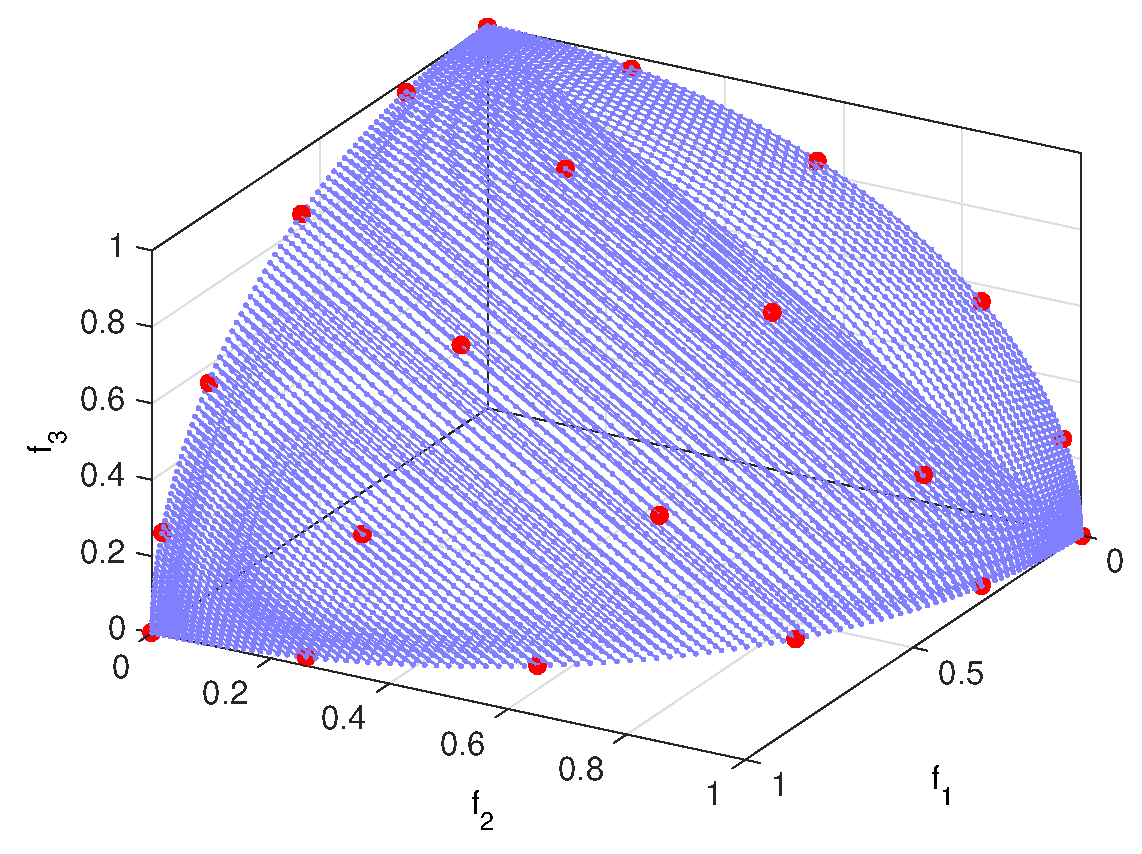
\includegraphics[scale=0.30]{dtlz2_original.eps}
	\caption{Pareto front for DTLZ2}
	\label{fig:dtlz2_original}
\end{figure}

The proposed approach to obtain the interpolated outcomes is discussed next. We refer to the method as Pareto linear interpolation~(PLI). The pseudo-code of PLI is given in Algorithm~\ref{alg:PLI}, followed by description of its key components. 

\begin{algorithm}[!ht]\footnotesize
	\caption{The proposed Pareto linear interpolation~(PLI) method}
	\begin{algorithmic}[1]
		\REQUIRE $PF$~(Given set of Pareto optimal outcomes), $|W|$~(Number of reference directions) \\	 
		\STATE \textbf{Create} all possible unique $M-1$, $M-2$,$\ldots$,$0-$\textcolor{blue}{simplexes having every vertex as a subset of the given Pareto optimal outcomes}
		\STATE \textbf{Apply} point-\textcolor{blue}{simplex} dominance rule to eliminate certain \textcolor{blue}{simplexes}
		\STATE \textbf{Generate} $|W|$ uniform reference directions using systematic sampling~\cite{DASAugust1998}
		\STATE \textbf{Identify} points of intersection between each reference direction and all survived \textcolor{blue}{simplexes} 
		\STATE \textbf{Compute} metrics for each reference direction 
	\end{algorithmic}
	\label{alg:PLI}
\end{algorithm}

\subsection{Create \textcolor{blue}{simplexes}} Given a set~($PF$) containing $N$ Pareto optimal outcomes, all possible unique \textcolor{blue}{simplexes}  $M-1$, $M-2$ through to \textcolor{blue}{$0-$simplexes} is constructed, by selecting the corresponding number of vertices from $PF$. Hence, the number of \textcolor{blue}{$k-simplexes$} would be $N\choose {k+1}$. Here, $TP$ is used to denote the resulting set of all \textcolor{blue}{simplexes}. Thus, the total number of \textcolor{blue}{simplexes} in $TP$ can be calculated as:

\begin{equation}\small
\begin{aligned}
&\hspace{-1.5em}\left|TP\right| = \sum_{i = 1}^m{N\choose i}\\
\label{eqn:NP}
\end{aligned}
\end{equation}

\subsection{Apply elimination rule} 
Once the set of \textcolor{blue}{simplexes} $TP$ is constructed, \emph{point-\textcolor{blue}{simplex}} dominance rule is applied to each of them. A \textcolor{blue}{simplex} is eliminated if any point~(note: not only the vertices) in the \textcolor{blue}{simplex} dominates or is dominated by a point of the given Pareto optimal set $PF$. The application of the above rule results in a set of surviving \textcolor{blue}{simplexes}~($TP_s$). {\color{blue}The dominance comparison is exact in nature, performed by solving a linear programming~(LP) problem as done in \cite{hartikainen2011constructing}}. 

{\color{blue}
	It is worth revisiting here that PAINT uses three elimination rules, i.e., \emph{point-simplex dominance}~(R1.1), \emph{self-dominance}~(R1.2), and \emph{simplex-simplex dominance}~(R2), as described in Section~\ref{sec:intro}. In effect, we are only using R1.1 in the proposed approach. The reason behind not using the other two are explained below.  
	
	\subsubsection{Self-dominance~(R1.2):} This particular rule is used in PAINT to eliminate simplexes that are \textit{self-dominating}, i.e., there exists at least one point in the simplex that dominates another point on the same simplex. Evidently, such simplexes should be excluded from the final approximation set for it to be inherently non-dominated. However, the rule appears to be redundant since such eliminations are already covered by point-simplex dominance~(R1.1). It is not possible to have a simplex where an internal point dominates another \emph{and} no vertex dominates any internal point. Thus, point-simplex check \emph{includes} self dominance check. 
	
	Let's first look at the above assertion for the highest order simplexes in the initial set. For an $M-$objective problem, the initial set for PAINT contains $M$-simplexes which will never exist in the final set, \textit{because a POF can be at most an $(M-1)$-dimensional manifold}. For a 3-objective problem, this would be a set of 3-simplexes, i.e., tetrahedrons. Evidently, it could be seen that it is always possible to find two internal points in the volume of the tetrahedron such that one dominates the other. Thus, these could be eliminated outright without applying the self-dominance rule -- or for that matter any of the rules discussed. 
	
	Next, let us look at the simplexes of degree $<M$. Consider a 2-simplex for a 3-objective minimization problem shown in Figure~\ref{fig:illus_r1}, constructed using points $P_1=(1,1,0.5),P_2=(0.4,0,0),P_3=(0,0.4,0)$. An internal point $PI_1=(0.21,0.43,0.075)$ in the simplex dominates another point $PI_2=(0.424,0.424,0.14)$. Let us assume that none of the vertices dominate or are dominated by any point in the simplex. Now, consider the direction vector formed by joining these two points ($PI_1$ and $PI_2$), referred to here as ``dominance direction''. It is evident that no two unique points along this direction could be non-dominated. Now construct vectors parallel to the dominance direction passing through each of the vertices. If the assumption above is true, then it implies that no points of the simplex exist along these vectors~(other than these vertices). For this to be true, the simplex must be non-convex. However, it is not possible to construct a non-convex simplex using $M$~(or fewer) points in $M$ dimensions~($M=3$ in this case), which is a contradiction. Thus, there must exist some points which at least one of the vertex dominates or is dominated by. In Figure~\ref{fig:illus_r1}, it can be seen that along the dominance direction, $P_1$ and $P_2$ do not dominate any point, but $P_3$ does. Hence, the simplex could be eliminated using \textit{point-simplex}~(R1.1) rule instead of self dominance. It could be further inferred that the same will also hold for all simplexes of order $<(M-1)$, since they are simply subsets of the $(M-1)$-simplexes. Given this property, the self dominance rule is not required. Also, the proposed method PLI only generates simplexes of order $<(M-1)$ as part of the initial set~(as discussed earlier in this section).
	
	\begin{figure}[!htb]
		\centering
		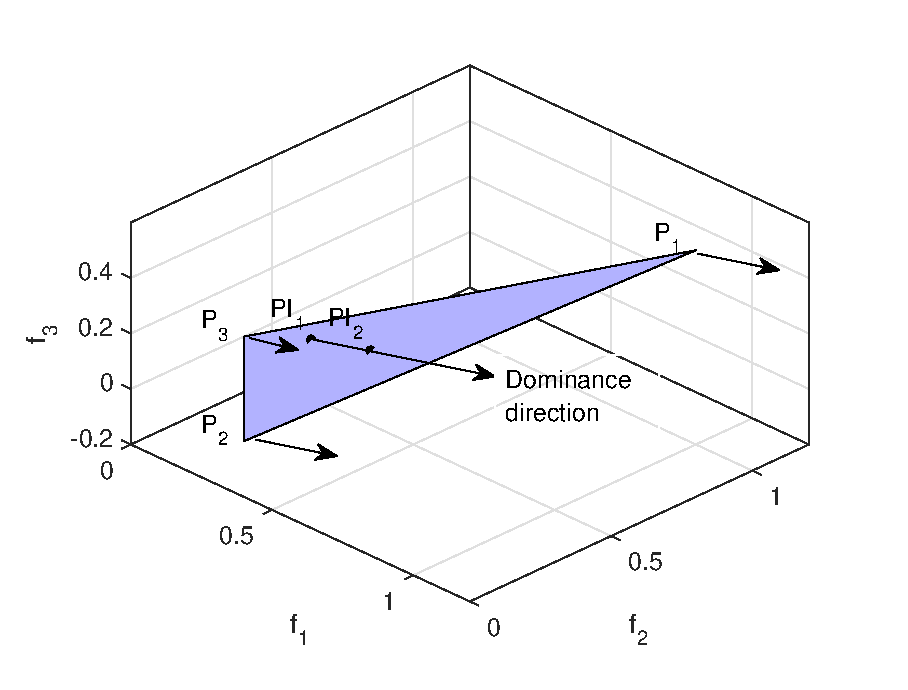
\includegraphics[width=.40\linewidth]{illus_r1.eps} \vspace{1em}
		\caption{Self dominance and point-simplex dominance}
		\label{fig:illus_r1}
	\end{figure}
	
	\subsubsection{Simplex-simplex dominance:}
	
	This rule has been used in PAINT because inherently non-dominated set was sought as the final result. However, as discussed in Section~\ref{sec:intro}, enforcement of inherent non-dominance may eliminate certain useful simplexes. Therefore, this rule is not used in the proposed approach. 
	
	It can be further noted that the output of the proposed elimination is independent of the order in which comparisons are done, which makes the approach amenable to parallelization. This means that even though the initial set of {\color{blue}simplexes} may be larger than that used in PAINT, the run-time could be reduced significantly by performing the comparisons in parallel. The advantage gained in doing so will vary depending on the number of nodes available and the relative complexity of solving LP problems v/s communication between the nodes. 
}
\subsection{Generate reference directions} Once the set of surviving {\color{blue}simplexes} $TP_s$ is identified, a uniformly spread set of interpolated outcomes is sought belonging to $TP_s$ to offer diverse additional choices to the DM. To achieve this, a structured set $W$ reference points is generated spanning a hyperplane with unit intercepts in each objective axis~(obtained by normalizing each objective between 0 and 1). This systematic sampling method is known as Normal Boundary Intersection (NBI)~\cite{DASAugust1998}. The use of NBI to generate such directions is appropriate given that it is at the core of most current decomposition based evolutionary algorithms~\cite{Asafmany2015}. It generates $|W|$ points on the hyperplane with a uniform spacing of $\delta=1/s$ for a given number of objectives $M$ with $s$ unique sampling locations along each objective axis. The total number of reference points~$|W| = {M+s-1\choose s}$. The distribution of the reference points is presented in Figure~\ref{fig:Refpoint} for a problem with three objectives~($M=3$) and a spacing parameter $s=5$. The idea behind generating this structured set of points to create reference direction vectors by joining them to the ideal point~(origin in the scaled space). A good multi-objective approximation would contain a representative solution along~(or close to) each of these uniformly distributed directions. This concept is used for evolutionary search in some of the prominent contemporary algorithms, especially for \emph{many-objective} optimization problems~\cite{Asafmany2015}. {\color{blue}Please take note that NBI method is not guaranteed to map all types of Pareto fronts perfectly~\cite{DASAugust1998}. Especially for a non convex frontier shape, the edges are difficult to map by using this method. However, the method is still able to generate relatively uniform points within a given resolution~(even though it might miss the exact edges), which makes it a preferred choice for most contemporary multi-/many-objective evolutionary algorithms.}


\begin{figure}[!ht]
	\centering
	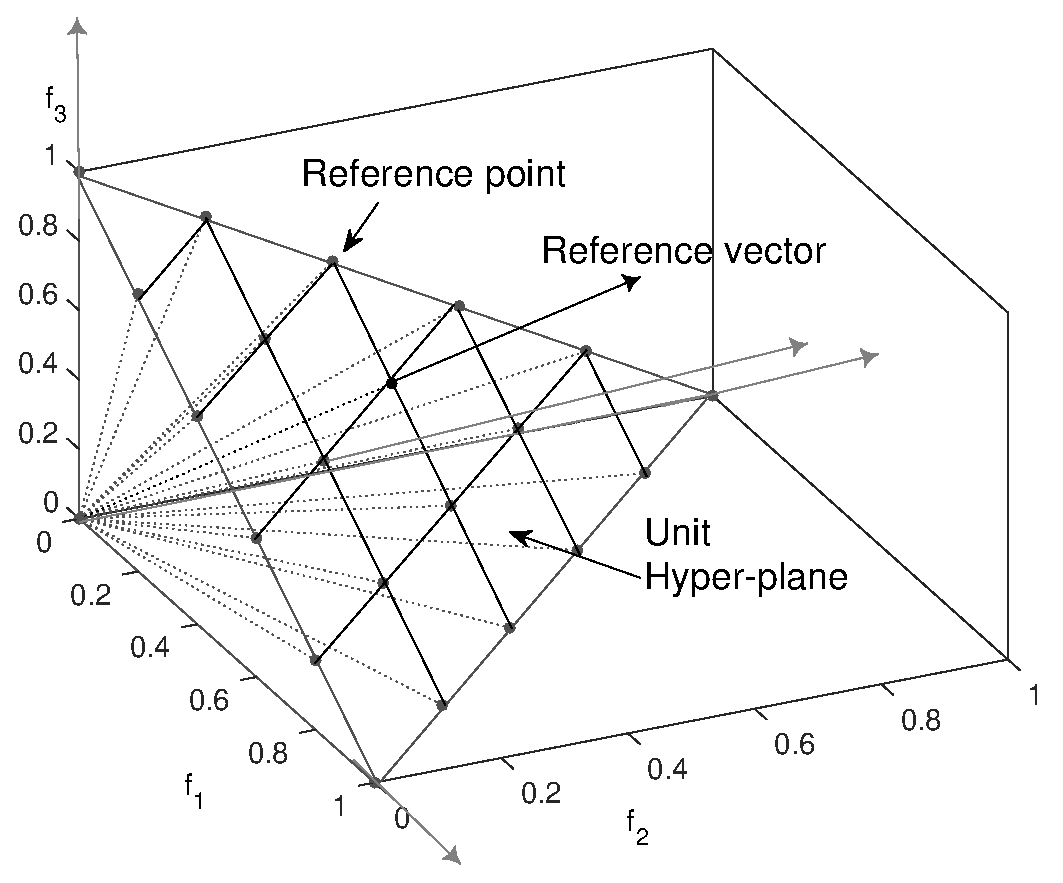
\includegraphics[scale=0.3]{StructureRefPoint.eps}
	\caption{A set of reference points for $M=3$ and $s=5$. }
	\label{fig:Refpoint}
\end{figure}



\subsection{Identify outcome(s) along each reference direction:} In order to determine the point of intersection between each reference direction and the surviving {\color{blue}simplexes} ~($TP_s$), the vertices of the {\color{blue}simplexes} are first normalized with respect to the Ideal and Nadir points. The point of intersection between a reference direction $\textbf{w}$ and a {\color{blue}$(k-1)-simplex$} defined using vertices $v_1,\dots,v_k$ can then be obtained by solving the linear programming problem~(LP) presented in Equation~\ref{eq:lp_exact}.

\begin{equation}\small
\begin{aligned}
\operatorname{Find} \; & \underset{i=1,\dots,k}{\alpha_i},\beta\\
& \text{such that}\\
& \sum_{i = 1}^k \alpha_i = 1,\\
& {\left(\sum_{i = 1}^k \alpha_iv_i\right)}_j = {(\textbf{w}\beta)}_j,~\forall~j = 1,\dots,M \\
& \text{where}\\
& \alpha_i~\in~[0,1],~\forall~i = 1,\dots,k,\\ 
& \beta~\in~(0,\infty),\\  
\label{eq:lp_exact}
\end{aligned}
\end{equation}

The above problem is solved for each direction against each {\color{blue}simplex}, executed in parallel for minimal run-time. A feasible solution to the above LP corresponds to one interpolated outcome in $TP_s$ for a direction. The intersection point in this case will be ${\left(\sum_{i = 1}^k \alpha_iv_i\right)}_j,\;\forall j = 1,\dots,M$. It is important to highlight that there may be more than one interpolated points along a given reference direction. For the three objective DTLZ2 problem discussed earlier, several reference directions could have one interpolated point on the inner face and one on the outer face as depicted in Figure~\ref{fig:dtlz2_intersection}. If for any reference direction, there are no feasible solutions obtained using the above LP, it may indicate a potential void in the Pareto outcome space. Such a void could be a manifestation of discontinuities in the front~(for example, due to constraints) or degeneracy in the front~(e.g. DTLZ5), both of which are analyzed later in the paper.

\begin{figure}[!ht]
	\centering
	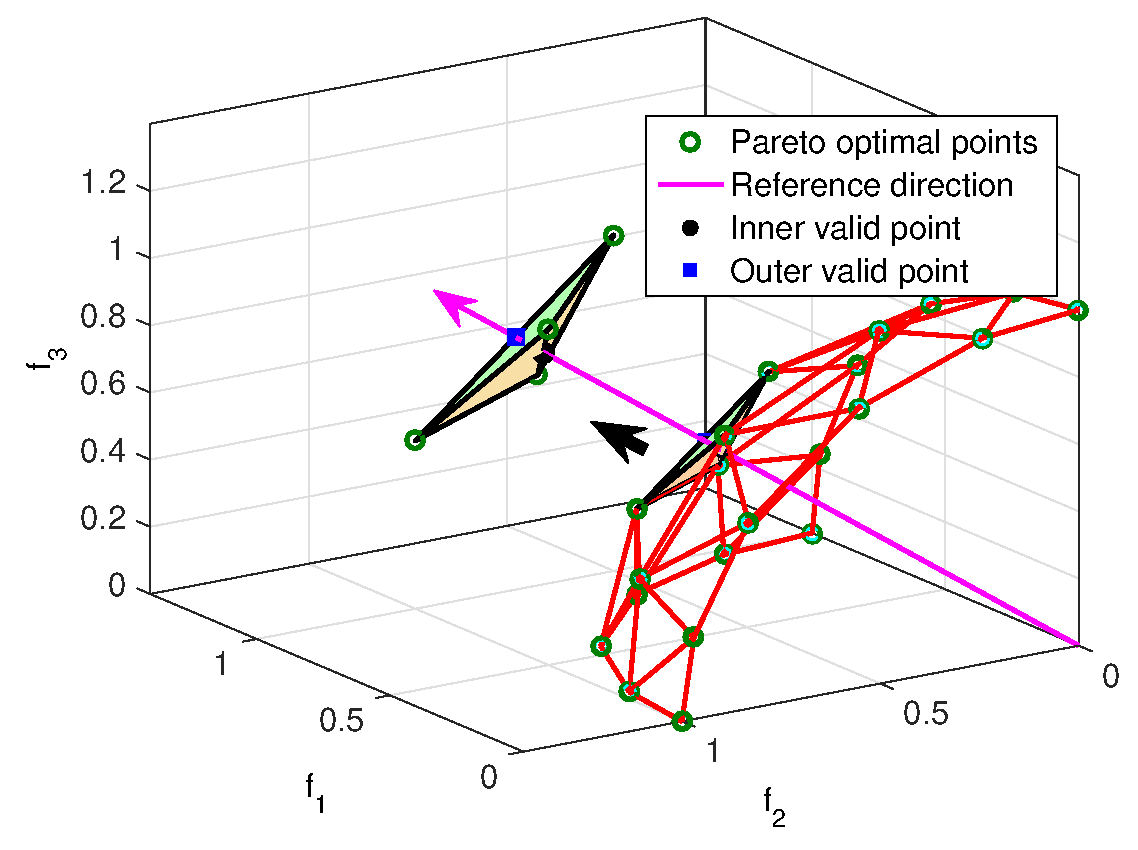
\includegraphics[width=0.40\linewidth]{dtlz2_valid_intersection.eps}
	\caption{Intersections along a reference direction}
	\label{fig:dtlz2_intersection}
\end{figure}

\subsection{Compute metrics:} Since the additional outcomes are generated using interpolation of the given Pareto optimal outcomes, they are not guaranteed to be Pareto optimal for the original problem, even though they are non-dominated with the given Pareto outcomes. However, it is important to quantify merits associated with the interpolated outcomes, as this information is useful for determining confidence on these outcomes during decision making. Two metrics are considered in this study to quantify the merit: dominance measure and nearest neighbor distance. 
These are discussed briefly below. {\color{blue}Note once again that these measures are calculated within a normalized space~(between 0 and 1 using the limits of $PF$), so that each objective is treated equally irrespective of the order of absolute values.} 
{\color{blue}
	\begin{enumerate}
		\item \emph{Dominance measure:} Given an interpolated point~(after the linear approximation has been constructed) this metric determines the minimum amount required to be subtracted from it to dominate or added to it to be dominated by a Pareto optimal outcome in the given set $PF$. In this paper, positive dominance measure~(Figure~\ref{fig:posdom}) is quantified as the minimum value when added to any one of the objectives of an outcome, it will be dominated by at least one of given Pareto outcomes. On the other hand, negative dominance measure~(Figure~\ref{fig:negdom}) of an outcome is the minimum value to be subtracted in any one of the objectives in order to dominate at least one given Pareto outcome. 
		
		It is worthwhile noting here the significance of the positive and negative dominance measures defined above. In literature, a subclass of linear interpolation methods is the so called \textit{Sandwich approximation}~\cite{ruzika2005approximation}. A sandwich approximation typically is a superposition of \textit{inner} and \textit{outer} approximations, between which the Pareto solutions are is bounded. A number of different types of sandwich approximation methods exist, 
		some of which create rectangular bounds~\cite{payne1993efficient}. The dominance errors presented above essentially represent the distance to the nearest rectangular bound. More specifically, the positive dominance measure defines the nearest distance to the worst case approximation and the negative dominance measure defines the nearest distance to the best case approximation. A part of the best case and worst case approximations could thus be constructed by translating the interpolated points along these minimum distances. For example, in Figure~\ref{fig:posdom}, if the interpolated outcome is translated along $d1$, an outcome on the worst case approximation could be obtained. Similarly, if the interpolated outcome in Figure~\ref{fig:negdom} is translated along $d2$, an outcome on the best case approximation could be obtained. In-fact, if these positive and negative dominance measures are further considered in \emph{each objective individually}, then the entire worst case and best case approximations could be constructed using the given interpolations. 
		
		
		\item \emph{Nearest neighbor distance:} While the above metric might be useful in quantifying the merit of an interpolated outcome, they cannot guarantee~(or capture probability of) the existence of that outcome along a reference direction. Therefore, in order to provide further insights for better decision making, we propose a second metric, termed as the \emph{nearest neighbor distance}. It measures the shortest Euclidean distance of an interpolated outcome along a reference direction to its nearest Pareto outcome, as shown in Figure~\ref{fig:mindist}. A large value of this metric would suggest lower confidence in existence of a solution along that direction, since the nearest Pareto outcomes are far away from it. It might be possible that no solutions exist in the Pareto front along that direction, which might be due to {\color{blue}degeneracy or a void/discontinuity}. 
	\end{enumerate}
}

Overall, the above two metrics determine the quality of the interpolated outcomes along any direction, which is useful when these outcomes are used in further endeavors. For example, if used as a reference point for evolutionary search, an interpolated outcome with large dominance measure and/or a large nearest neighbor distance metric could be considered relatively risky as it amounts to search in an unexplored region {\color{blue}(large difference between worst case and best case approximation)} with a large range of variation in performance. Therefore choosing an outcome with low values of these metrics is likely to deliver a true solution along the direction. {\color{blue}On the other hand these unexplored regions can also be considered as valuable, because they are not sufficiently sampled. Although the quality of the interpolated outcomes can be derived from the metrics, the final decision remains with the DM, who is better informed in any case.} 


\begin{figure*}[!ht]
	\centering
	\subfigure[Positive dominance error]{\label{fig:posdom}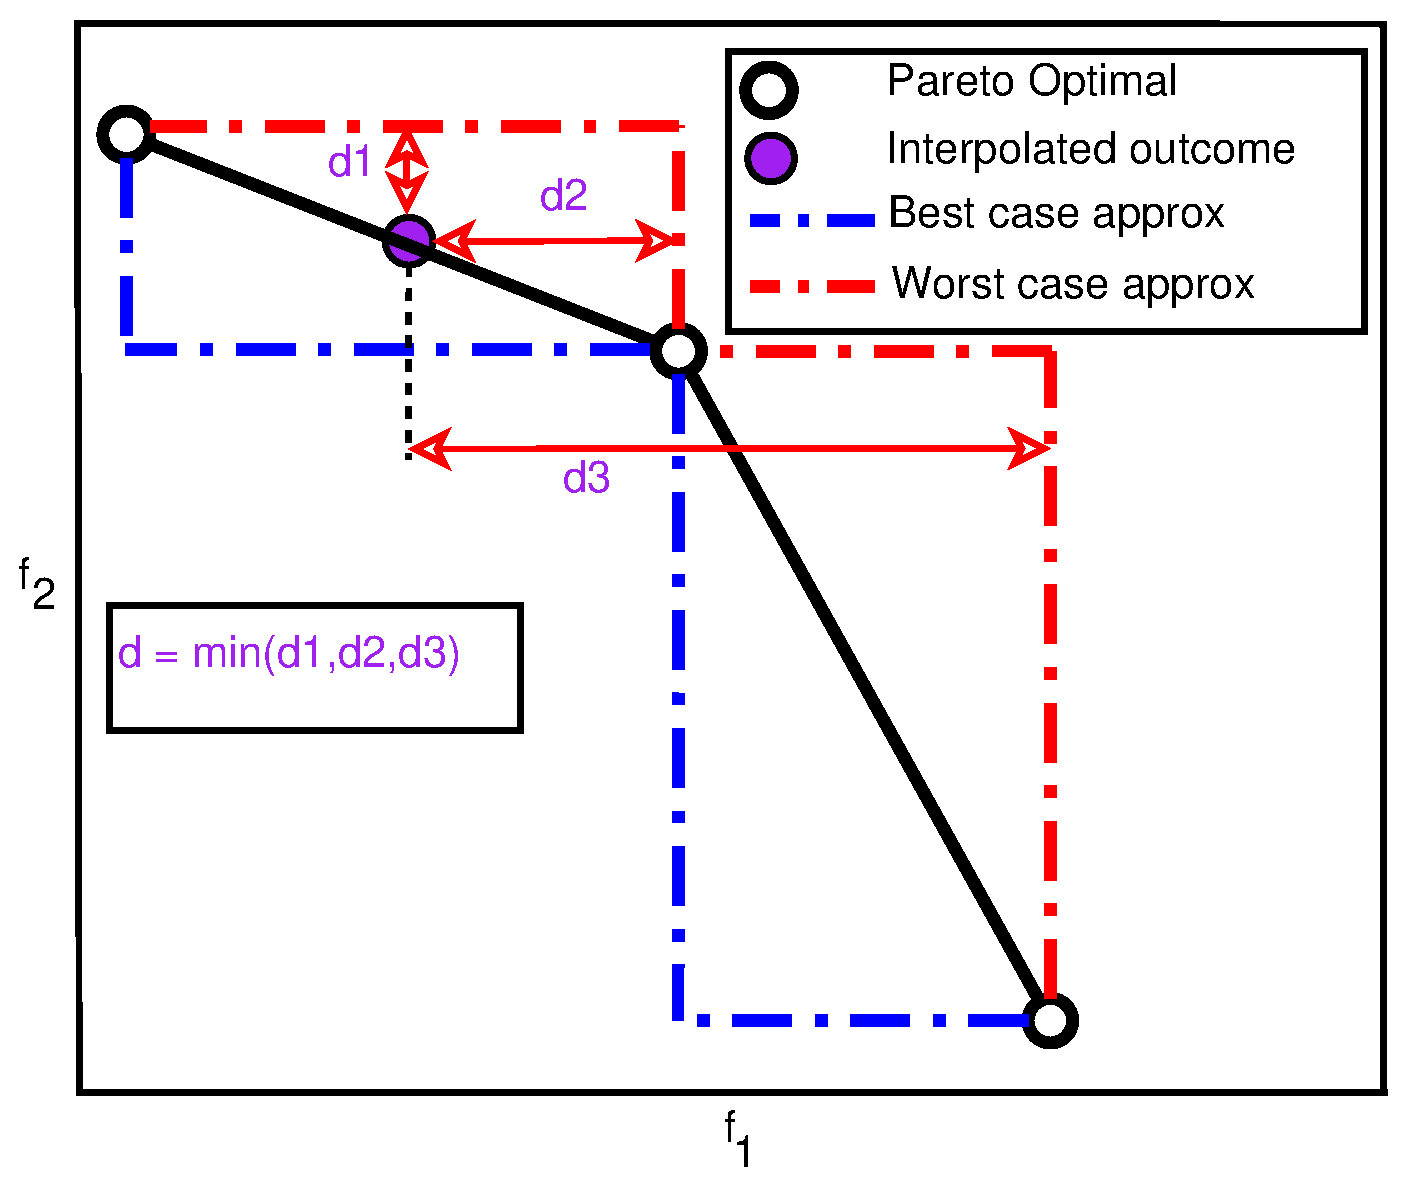
\includegraphics[width=.303\linewidth]{posdom.eps}}
	\subfigure[Negative dominance error]{\label{fig:negdom}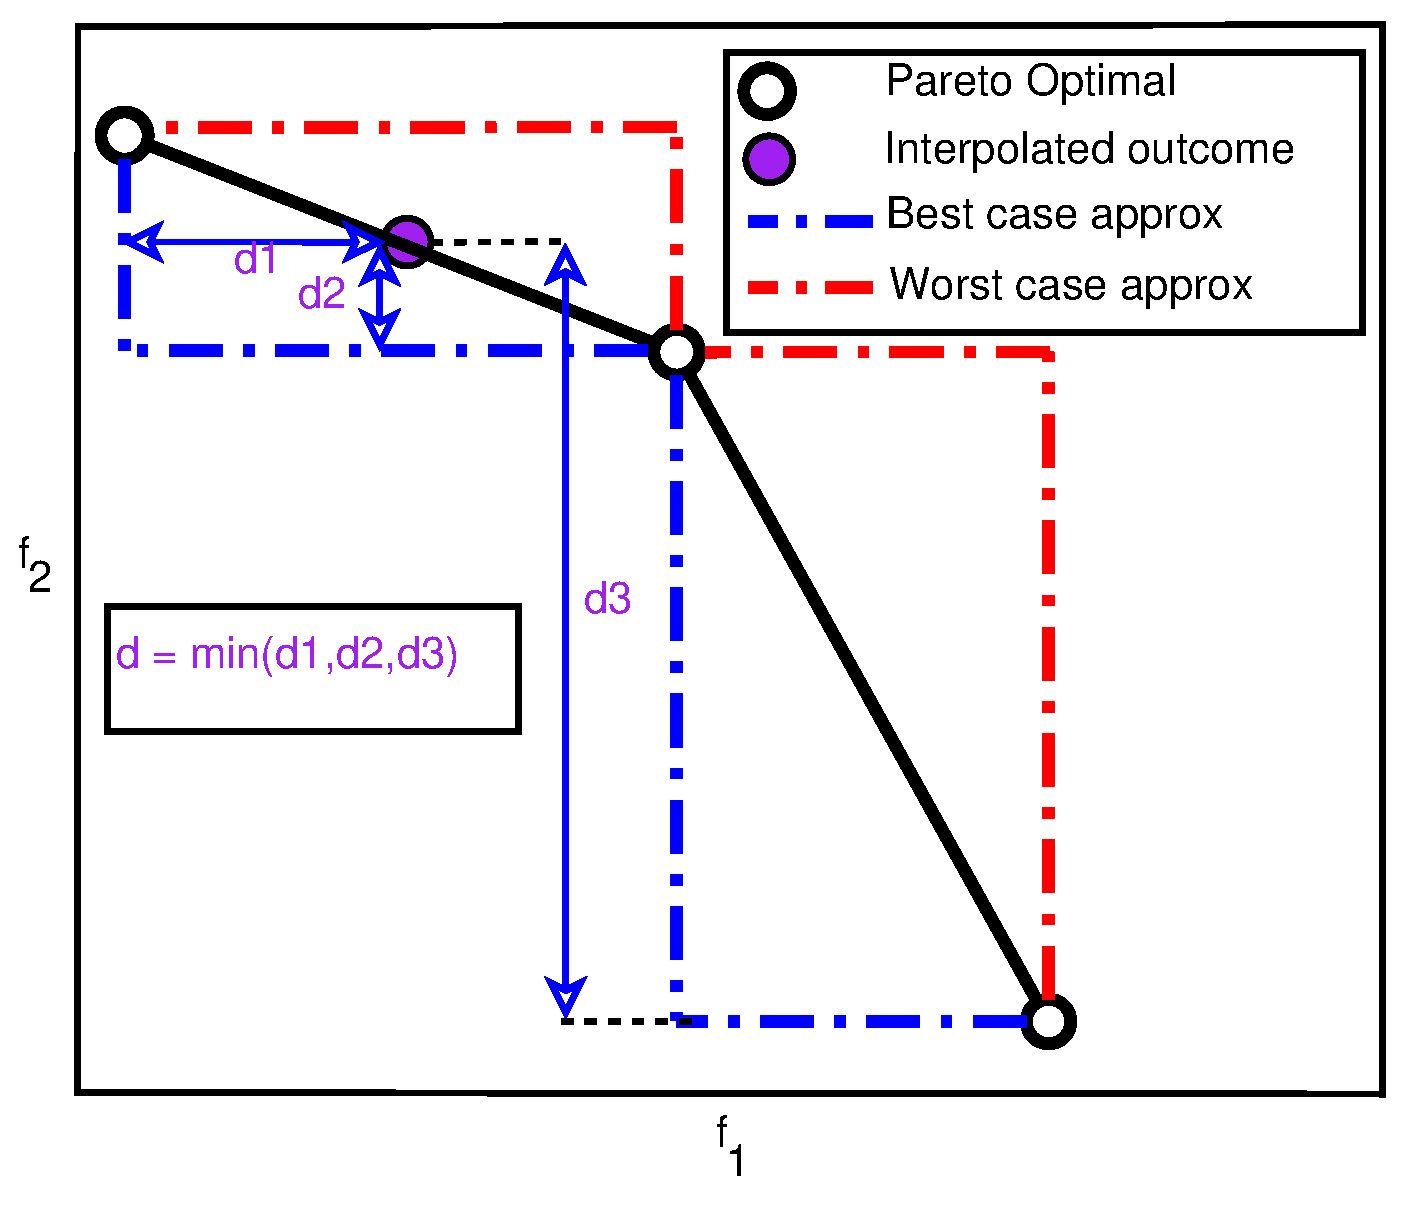
\includegraphics[width=.30\linewidth]{negdom.eps}}
	\subfigure[Nearest neighbor distance]{\label{fig:mindist}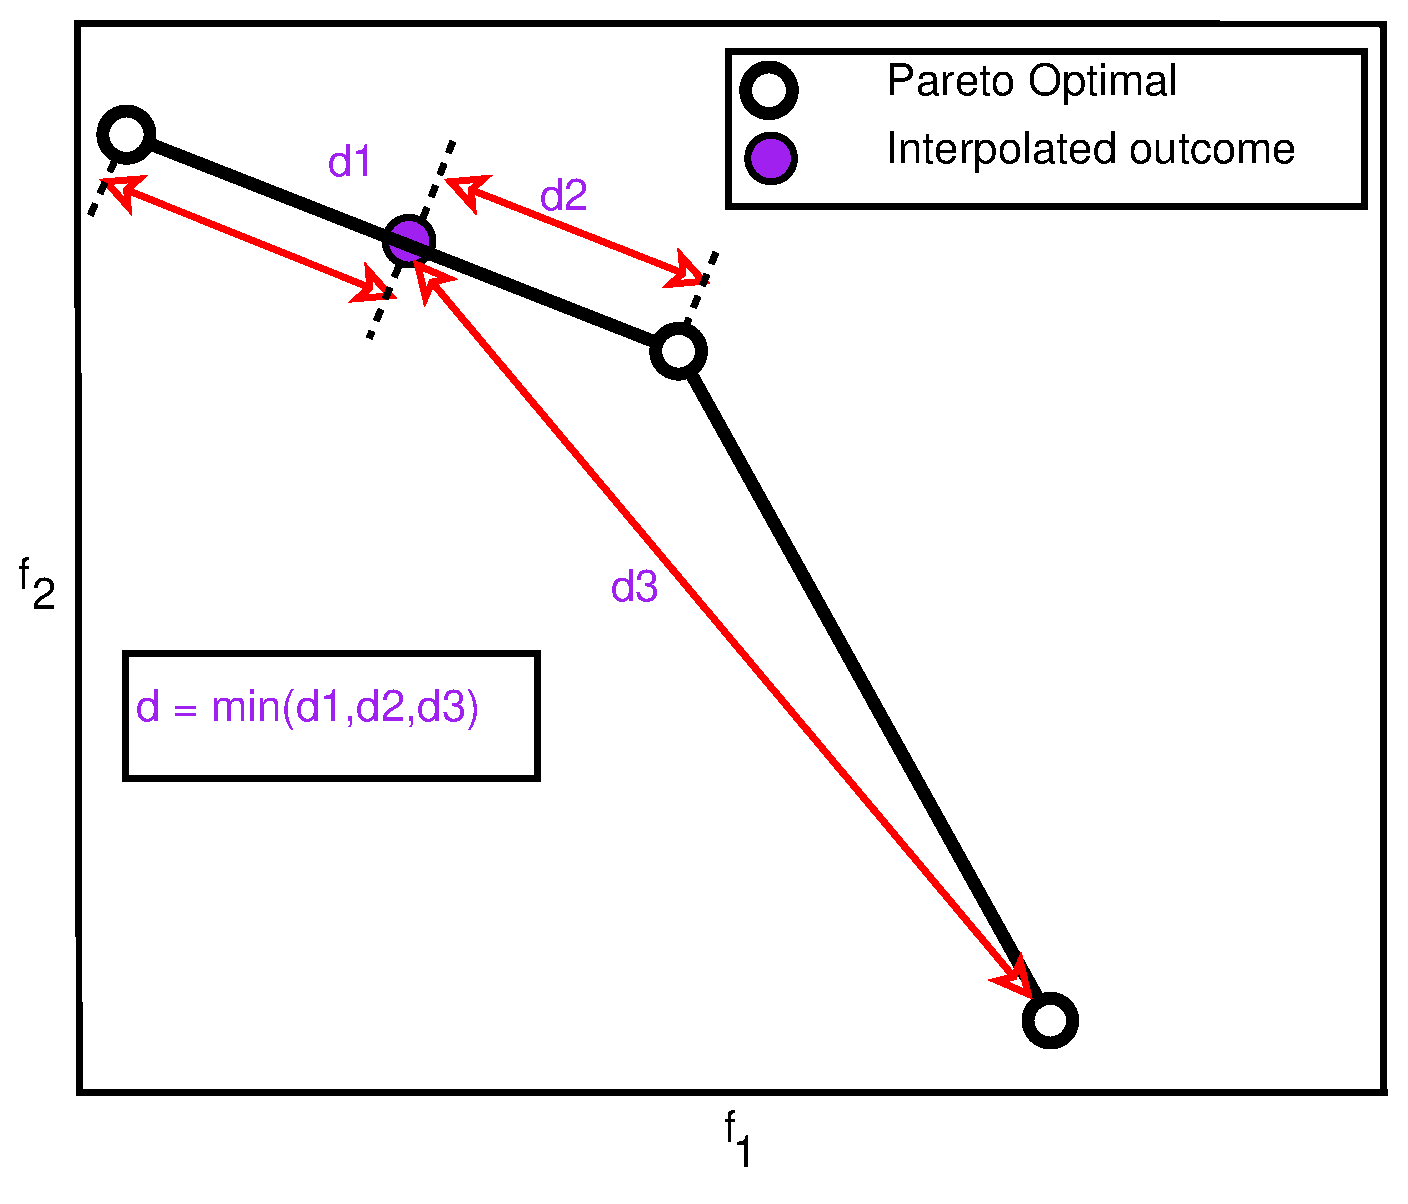
\includegraphics[width=.303\linewidth]{mindist.eps}}
	\caption{Metrics}
	\label{fig:metric}
\end{figure*}

{\color{blue}
	\subsection{Computational Complexity}
	Let us consider the relative complexity of the presented algorithm~(PLI) as compared to PAINT. As discussed in \cite{hartikainen2012paint}, the complexity includes the construction of the Delaunay triangulation, and the dominance checks. The complexity of Delaunay triangulation for $N$ points in $M$ dimensions to generate initial simplexes is $O((M+1)c_n/N)$, where $c_n=O(N^{{\left\lfloor (M+1)/2\right\rfloor}}/\left\lfloor (M+1)/2\right\rfloor!)$. However, dominant complexity step for PAINT algorithm is not this, but the simplex elimination process. For PAINT, the number of initial simplexes can be at most $O(N^{\left\lceil  M/2\right\rceil})$. This implies that in the worst case, $O(N^M)$ comparisons need to be made~\cite{hartikainen2012paint}. Each of these comparisons are done by solving a linear programming problem, whose complexity depends on $M$ and the size of simplex(s) involved in comparison. The resulting LP problems are reasonably small-sized, so all these problems are considered equivalent. Thus the worst case complexity of PAINT is considered as $O(N^M)$. Now, in PLI, the Delaunay triangulation is not required, so the computational expense involved is only in selection of points, which is negligible. Subsequently, each given outcome is compared with each simplex, so the resulting complexity is $O\left(N \times \left[\sum_{i=2}^M {N \choose i}\right]\right)$. The difference in computational complexity for 20, 40, and 60 given Pareto optimal outcomes up to 15 dimensions are shown in Figure~\ref{fig:complexity}. It can be concluded that up to 4 dimensions PAINT is less computationally expensive than PLI for each case. However for number of dimensions higher than 4, PLI has a remarkable computational advantage. For example, the worst case complexity of PAINT for involving 20 Pareto optimal outcomes in 6 dimensions is 64E06 whereas in the context of PLI it is only 1.20878E06, which is about 60 times less than PAINT. The comparisons done in PLI can also be parallelized, which can further reduce the complexity by a factor dependent on the computing infrastructure~(e.g. number of nodes).
	
	\begin{figure}[!ht]
		\centering
		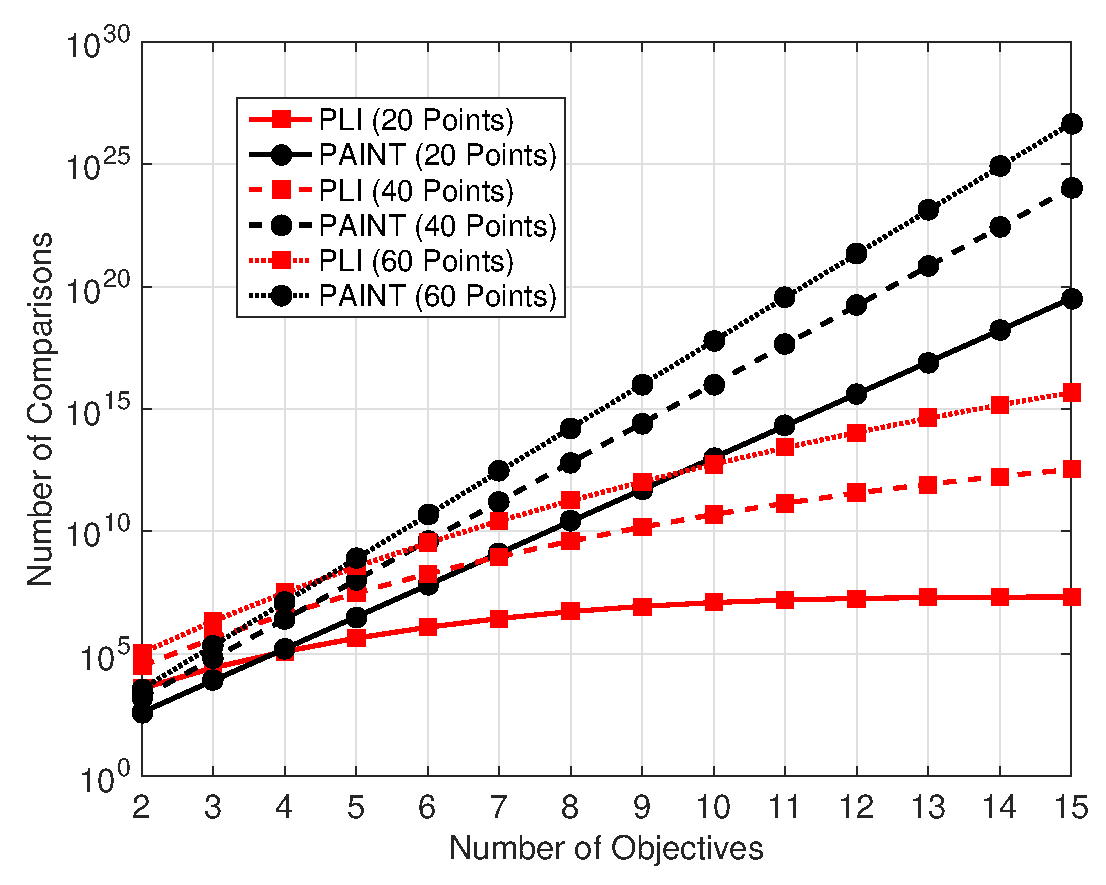
\includegraphics[width=0.40\linewidth]{Complexity.eps}
		\caption{Complexity comparison}
		\label{fig:complexity}
	\end{figure}
}

\section{Numerical Experiments}
\label{sec:numex}
In this section, we study the performance of the proposed approach using one bi-objective test example~($L\&H_{2\times 2}$), six well established tri-objective test problems~(DTLZ1, DTLZ2~(original and modified), WFG2, DTLZ5, DTLZ7, Hourglass) and two practical examples~(heat exchanger design and forest management) spanning intersecting local fronts, convex, {\color{blue}non-convex} and mixed fronts. The number of reference directions is set to $10$ for bi-objective problem and $300$ for all the tri-objective problems except for DTLZ5 for which $990$ reference directions were used. The given set of Pareto optimal outcomes for all the problems are available for download at this \href{http://www.mdolab.net/Ray/Research-Data/Polytope-dataset.zip}{\underline{link}}. 

{\color{blue}\subsection{Intersecting local fronts}
	We start with a bi-objective problem $L\&H_{2\times 2}$~\cite{hartikainen2014paint} involving two local non-convex fronts intersecting each other. In this problem the DM is provided with $7$ Pareto optimal outcomes. For this problem, all the initial simplexes are shown in Figure~\ref{fig:sicon_init}. The $PF$ corresponding to the final set of survived {\color{blue}simplexes} is presented in Figure~\ref{fig:sicon_approx}. The representative Pareto front (in light blue background) and the set of interpolated outcomes along $10$ uniformly distributed reference directions are presented in Figure~\ref{fig:sicon_all}. The negative and positive dominance measures are shown in Figure~\ref{fig:sicon_eps} and Figure~\ref{fig:sicon_reveps}. In contrast to \cite{hartikainen2014paint}, the proposed approach does not consider the effect of solution space~(decision space) while interpolation. As a result, the discontinuity in the front is not observed when using the proposed approach. }

\begin{figure*}[!ht]
	\centering
	\subfigure[]{\label{fig:sicon_init}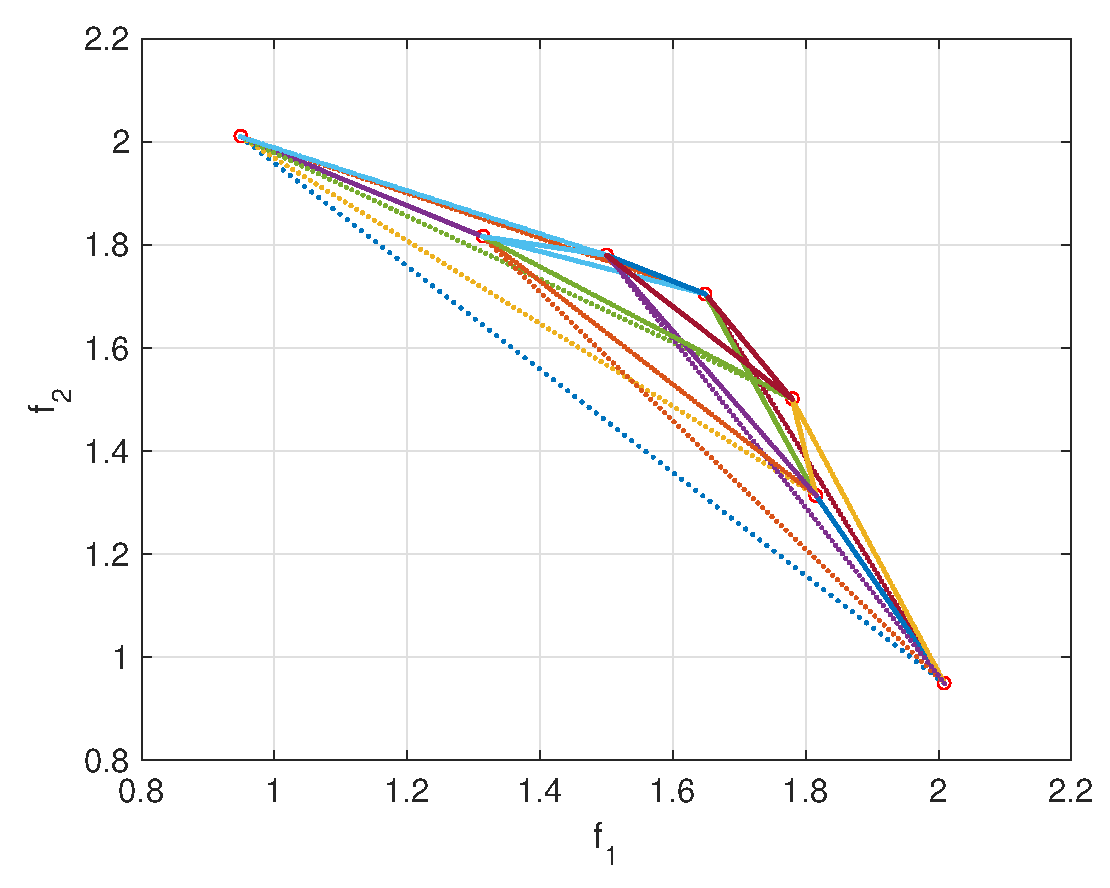
\includegraphics[width=.30\linewidth]{sicon_polytopeinit.eps}}
	\subfigure[]{\label{fig:sicon_approx}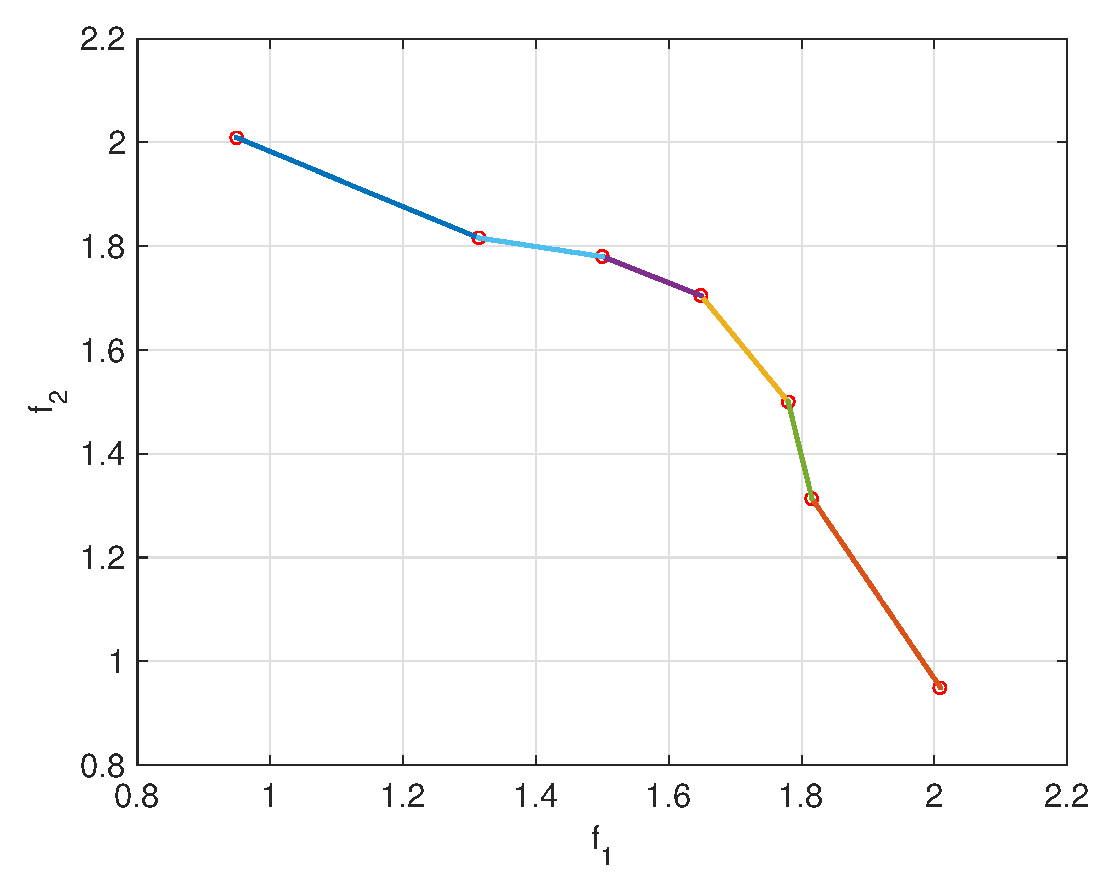
\includegraphics[width=.30\linewidth]{sicon_Approx.eps}}
	\subfigure[]{\label{fig:sicon_all}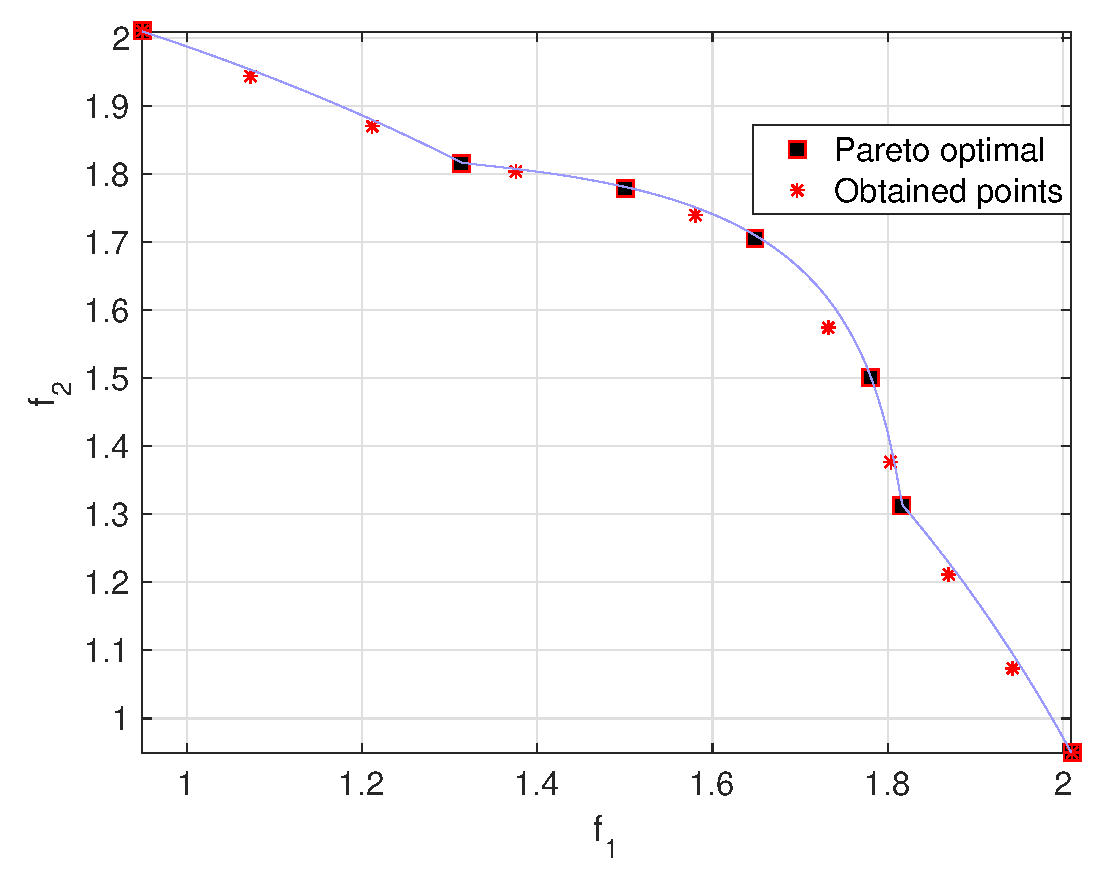
\includegraphics[width=.30\linewidth]{sicon_allpoint_10.eps}}\\
	\subfigure[]{\label{fig:sicon_eps}\includegraphics[width=.30\linewidth]{sicon_epsdom.eps}}
	\subfigure[]{\label{fig:sicon_reveps}\includegraphics[width=.30\linewidth]{sicon_epsrevdom.eps}}
	\subfigure[]{\label{fig:sicon_mindist}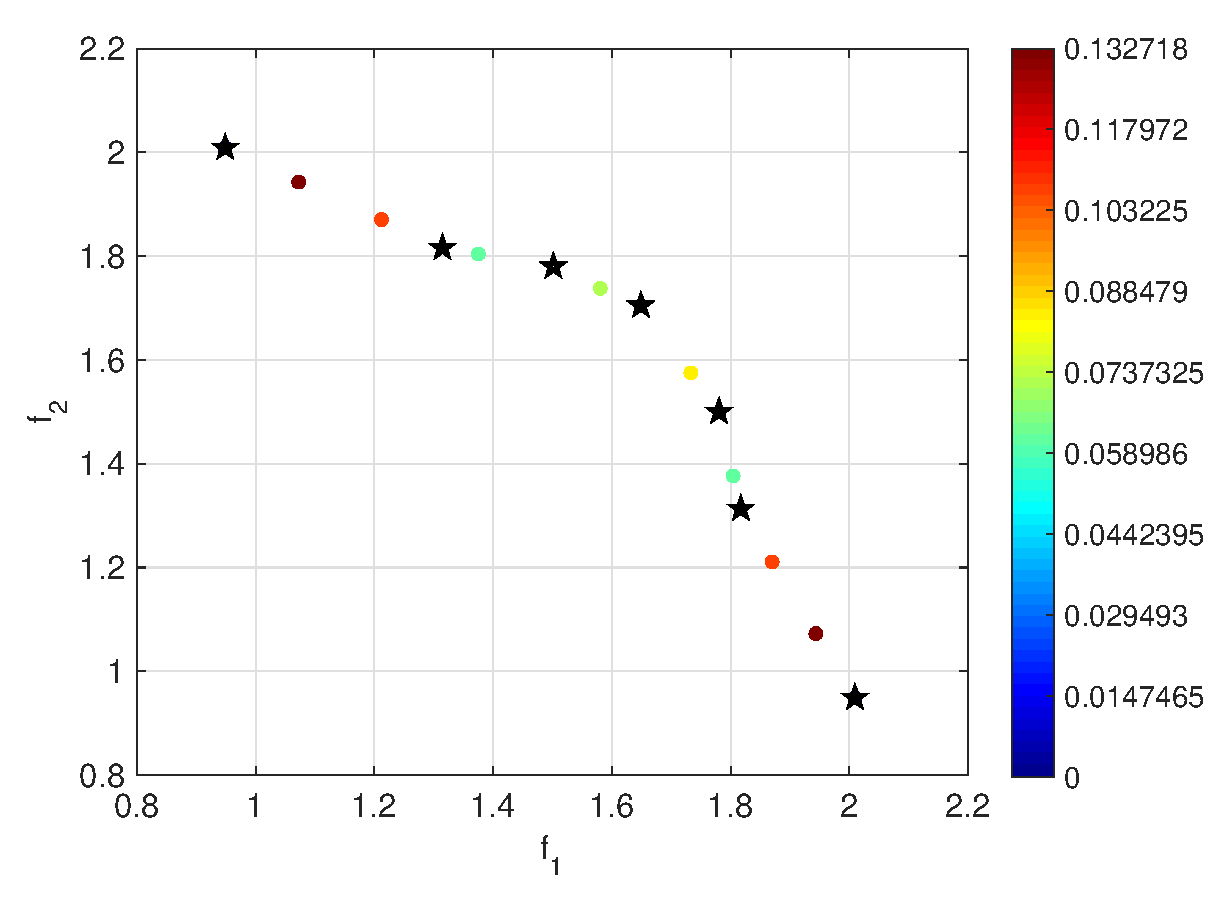
\includegraphics[width=.30\linewidth]{sicon_mindist_10.eps}}
	\caption{$L\&H_{2\times 2}$: (a) Set of initial {\color{blue}simplexes} (b) Survived {\color{blue}Simplexes} (c) Interpolated outcomes (d) Negative dominance measure (e) Positive dominance measure (f) Nearest neighbor distance}
	\label{fig:sicon_true_approx}
\end{figure*}

\subsection{Linear, Non-convex, Convex fronts} 
The $PF$ of the three objective DTLZ1 problem~\cite{deb2002scalable} is a planar surface and the DM is provided with $28$ Pareto optimal outcomes. This initial set of {\color{blue}simplexes} for this problem is shown in Figure~\ref{fig:dtlz1_3_init}. The $PF$ corresponding to the final set of survived {\color{blue}simplexes} is presented in Figure~\ref{fig:dtlz1_3_approx}. The theoretical Pareto front (in light blue background) and the set of interpolated outcomes along $300$ uniformly distributed reference directions are presented in Figure~\ref{fig:dtlz1_3_all}. The number of unique $1$ and $2-${\color{blue}simplexes} and the number of surviving $1-$ and $2-${\color{blue}simplexes}~(for these and all other problems discussed further) are listed in Table~\ref{tab:probstat}. For this problem, one can observe that there is only one interpolated outcome along each reference direction. {\color{blue}Notably, since the given Pareto outcomes lie on a plane and the Pareto front itself is planar all interpolated outcomes on each simplex will in-fact lie on the true Pareto front. Therefore, in the dominance comparisons, none of the given outcomes will dominate (or be dominated by) any of the interpolated points on any simplex. Consequently, there will be no eliminations, and the surviving simplex set may contain several overlapping simplexes}. To reduce the resulting redundancy, a non-overlapping set could also be identified among these. However, this is not a strictly essential step. A simple interpretation of the case is that it is possible to obtain a given interpolated point via several different possible sets of points~(which form vertices of the corresponding {\color{blue}simplexes}). {\color{blue}Take note that, this situation is strictly applicable only where the simplexes are contained on the same plane, e.g. in DTLZ1. This overlap will typically not occur for non-linear fronts, as will be observed in the next example(s). However, for completeness, it must also be noted that it’s possible to have highly unlikely cases where even for a non-linear front, all given set of Pareto outcomes are in the same plane. The proposed approach will interpret it as linear and construct similar overlapping approximations. In absence of any other information about the Pareto front, this will not be an anomaly since the method is based on interpolation alone.} 

\begin{figure*}[!ht]
	\centering
	\subfigure[]{\label{fig:dtlz1_3_init}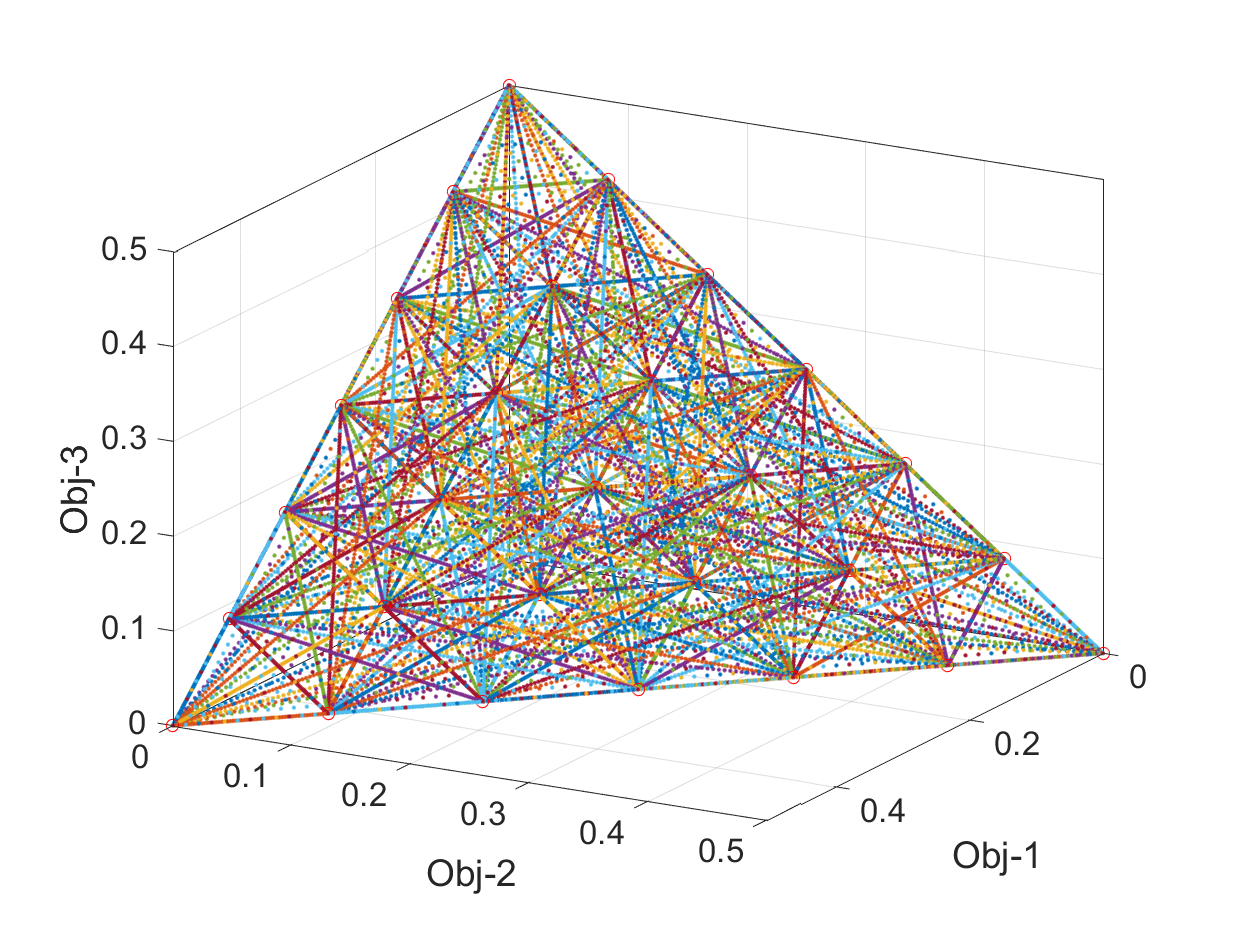
\includegraphics[width=.30\linewidth]{dtlz1_3_polytopeinit.eps}}
	\subfigure[]{\label{fig:dtlz1_3_approx}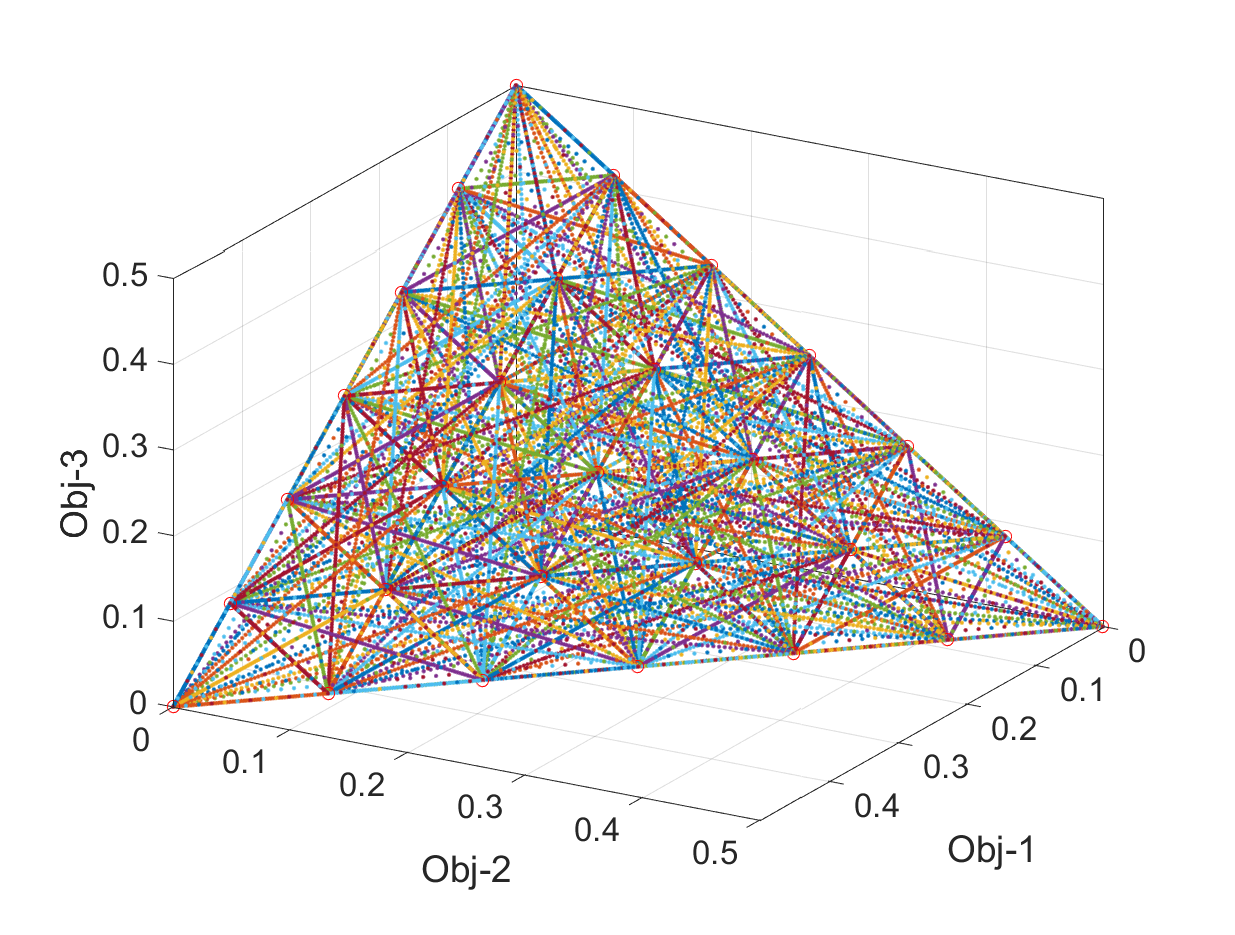
\includegraphics[width=.30\linewidth]{dtlz1_3_Approx.eps}}
	\subfigure[]{\label{fig:dtlz1_3_all}\includegraphics[width=.30\linewidth]{dtlz1_3_allpoint_300.eps}}
	\caption{DTLZ1: (a) Set of initial {\color{blue}simplexes} (b) Survived {\color{blue}Simplexes} (c) Interpolated outcomes}
	\label{fig:dtlz1_3_true_approx}
\end{figure*}

Next we present the results on three objective DTLZ2 problem~\cite{deb2002scalable}. The $PF$ is non-convex and the DM is provided with $21$ Pareto optimal outcomes. The initial and final set of {\color{blue}simplexes} are presented in Figure~\ref{fig:dtlz2_3_init} and Figure~\ref{fig:dtlz2_3_approx} respectively. The theoretical Pareto front (in light blue background) and the set of interpolated outcomes along $300$ uniformly distributed directions are presented in Figure~\ref{fig:dtlz2_3_all}. The number of unique $1$ and $2-${\color{blue}simplexes} and the number of surviving $1$ and $2-${\color{blue}simplexes} are listed in Table~\ref{tab:probstat}. For this problem our approach will preserve all possible {\color{blue}simplexes} that contain outcomes that are non-dominated with respect to the given Pareto optimal outcomes. Since we have already highlighted existence of inner and outer faces in Section~\ref{sec:intro}, we expect to observe multiple intersections for several weight directions. Among the 300 reference directions, all 300 of them have  outcomes~(some have multiple intersections) along them. 

\begin{figure*}[!ht]
	\centering
	\subfigure[]{\label{fig:dtlz2_3_init}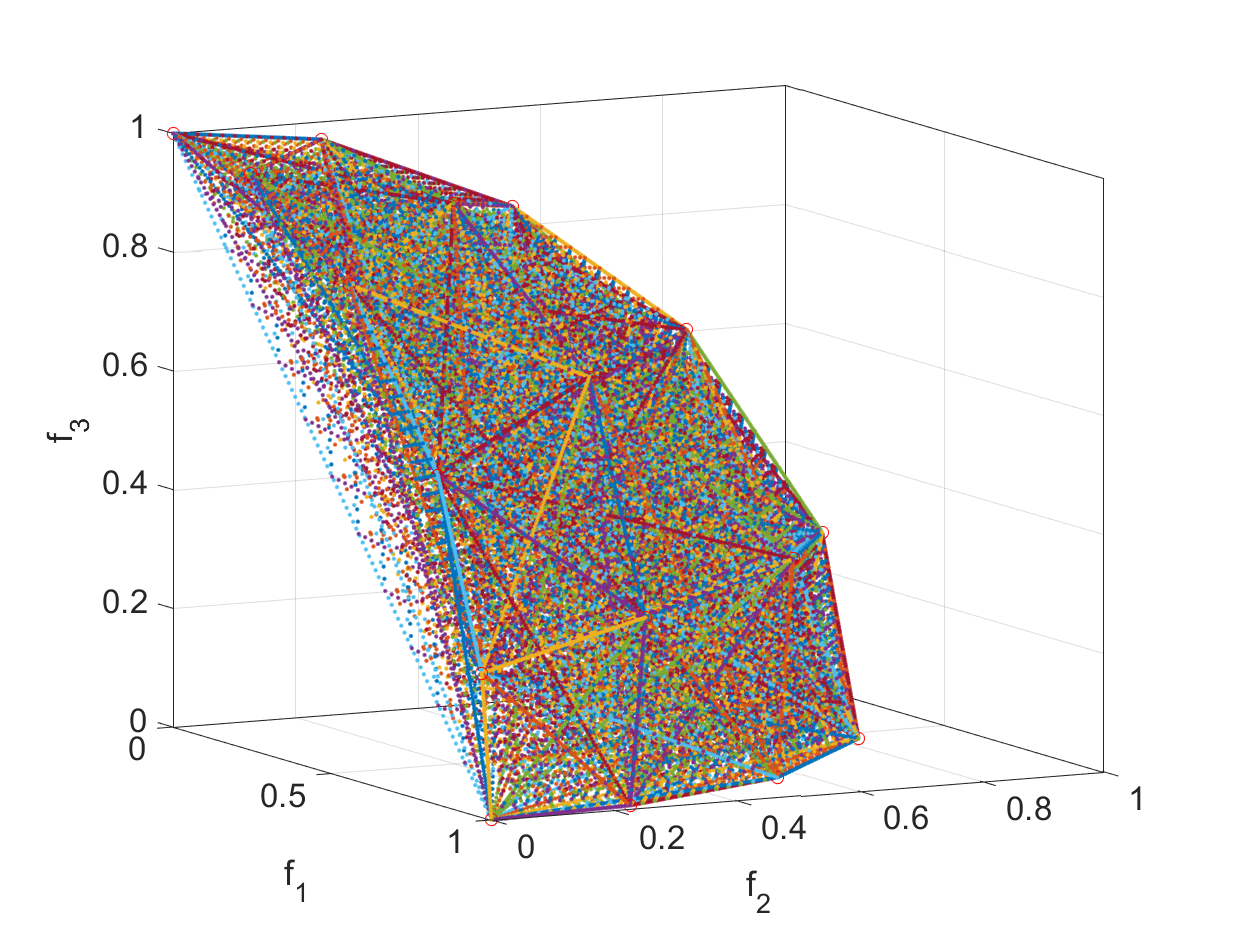
\includegraphics[width=.30\linewidth]{dtlz2_3_polytopeinit.eps}}
	\subfigure[]{\label{fig:dtlz2_3_approx}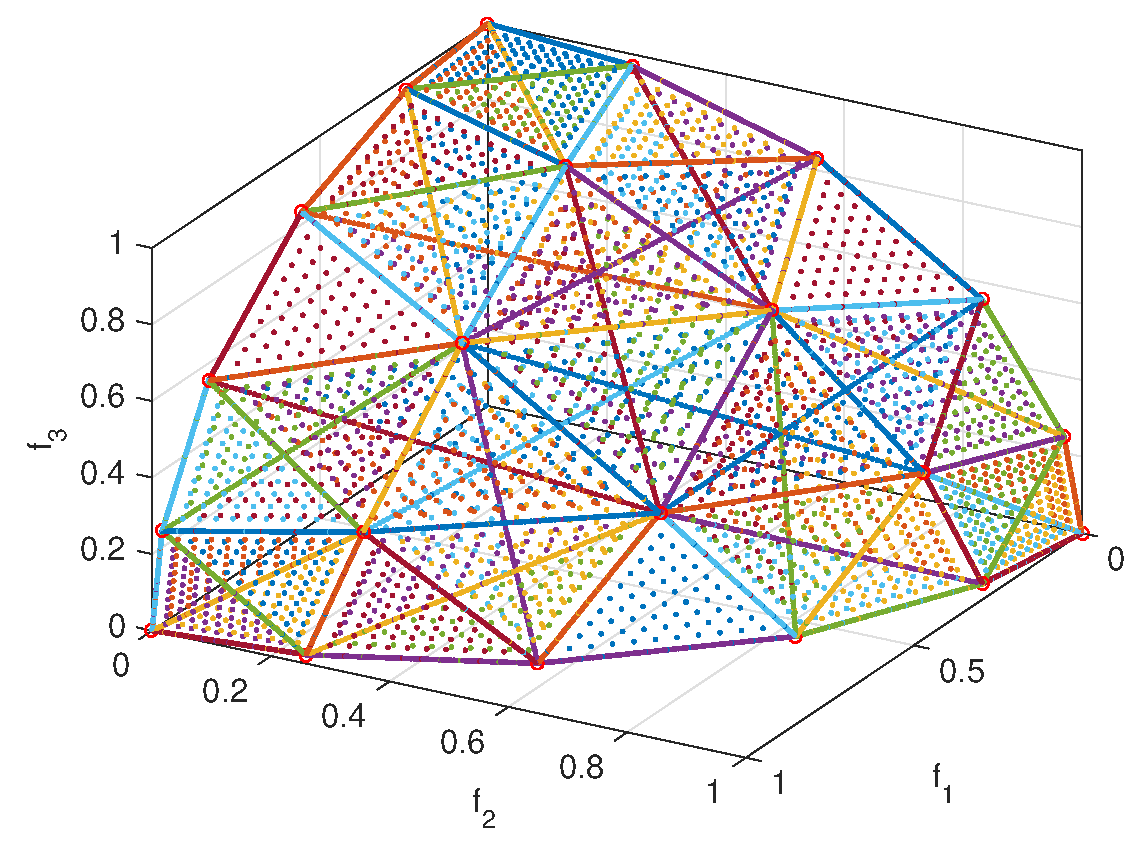
\includegraphics[width=.30\linewidth]{dtlz2_3_Approx.eps}}
	\subfigure[]{\label{fig:dtlz2_3_all}\includegraphics[width=.30\linewidth]{dtlz2_3_allpoint_300.eps}}
	\caption{DTLZ2: (a) Set of initial {\color{blue}simplexes} (b) Survived {\color{blue}Simplexes} (c) Interpolated outcomes}
	\label{fig:dtlz2_3_true_approx}
\end{figure*}

Next we illustrate the performance of the proposed approach on a problem with convex front, the three objective WFG2~\cite{huband_2006}. The initial set of {\color{blue}simplexes} are shown in Figure~\ref{fig:wfg2_init}, while Figure~\ref{fig:wfg2_approx} shows the final set of survived simplexes. The representative Pareto front (in light blue background) and the interpolated outcomes along every reference directions are shown in Figure~\ref{fig:wfg2_all}. Once again, multiple intersections are observed along several reference directions. For this problem, outcomes are obtained along $254$ reference directions. Including multiple intersections along several reference directions, the total number of unique outcomes is $1454$. {\color{blue}It is interesting to note that all the directions which did not have any solutions along them lay entirely in one of the planes~($f_1-f_2,f_2-f_3,$ or $f_1-f_3$). The reason is simply that the edge points of the Pareto front did not lie in these planes~(unlike DTLZ2). This is an example of the limitation of NBI method discussed earlier in Section~\ref{sec:approach}.} 

\begin{figure*}[!ht]
	\centering
	\subfigure[]{\label{fig:wfg2_init}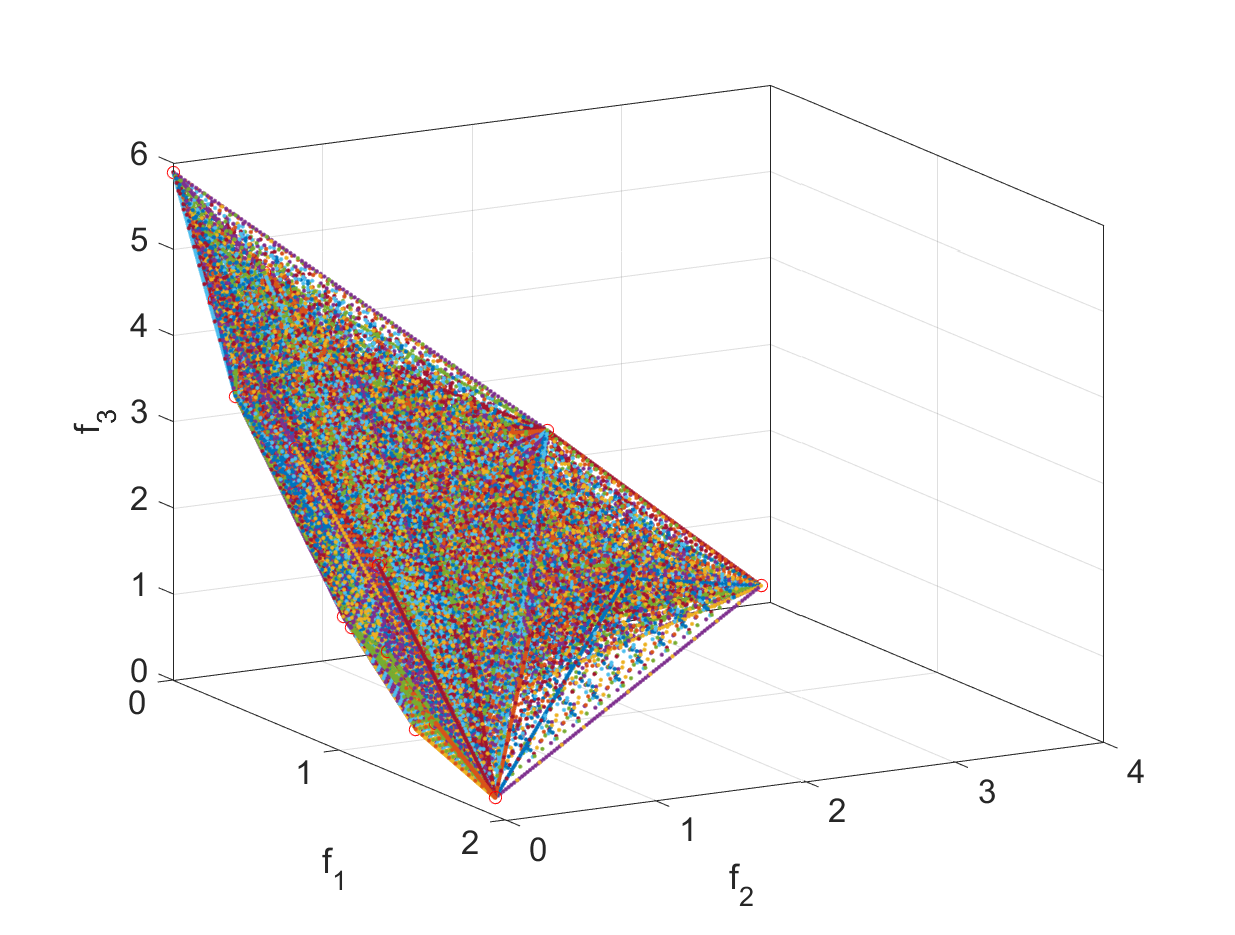
\includegraphics[width=.30\linewidth]{wfg2_polytopeinit.eps}}
	\subfigure[]{\label{fig:wfg2_approx}\includegraphics[width=.30\linewidth]{wfg2_Approx.eps}}
	\subfigure[]{\label{fig:wfg2_all}\includegraphics[width=.30\linewidth]{wfg2_allpoint_300.eps}}
	\caption{WFG2: (a) Set of initial {\color{blue}simplexes} (b) Survived {\color{blue}simplexes} (c) Interpolated outcomes}
	\label{fig:wfg2_true_approx}
\end{figure*}

\begin{table*}[!ht]\scriptsize
	\centering
	\caption{Statistics for all problems}
	\label{tab:probstat}
	\tabcolsep=0.11cm
	\begin{tabular}{llllllll}
		\specialrule{.1em}{.1em}{.1em} 
		{\bf Problem}           & {\bf $|PS|$} & {\bf {\color{blue}$|1-simplexes|$}} & {\bf {\color{blue}$|1-simplexes^{S}|$}} & {\bf {\color{blue}$|2-simplexes|$}} & {\bf {\color{blue}$|2-simplexes^{S}|$}} & {\bf $|IS|(|W|)$} & {\bf $|UI|(|W|)$} \\ \hline
		{\bf $L\&H_{2\times 2}$}             & 7                                & 21                     & 6                        & 0                    & 0                       & 10(10)                                                           & 10(10)                                                      \\ \hline
		{\bf DTLZ1}             & 28                                & 378                     & 378                        & 3276                    & 3276                       & 300(300)                                                           & 300(300)                                                      \\ \hline
		{\bf DTLZ2}             & 21                                & 210                     & 63                         & 1330                    & 61                         & 630(300)                                                           & 300(300)                                                      \\ \hline
		{\bf WFG2}              & 25                                & 300                     & 112                        & 2300                    & 148                        & 1454(300)                                                           & 254(300)                                                       \\ \hline
		{\bf DTLZ5}             & 5                                 & 10                      & 4                          & 10                      & 0                          & 22(990)                                                            & 22(990)                                                       \\ \hline
		{\bf DTLZ7}             & 12                                & 66                      & 38                         & 220                     & 57                         & 83(300)                                                           & 82(300)                                                      \\ \hline
		{\bf Hourglass}     & 55                                & 1485                    & 221                        & 26235                   & 257                        & 332(300)                                                           & 99(300)                                                       \\ \hline
		{\bf DTLZ2-mod}         & 28                                & 378                    & 128                         & 3276                    & 227                         & 1727(300)                                                           & 300(300)                                                      \\ \hline
		{\bf Forest management} & 20                                & 190                     & 82                         & 1140                    & 109                        & 534(300)                                                           & 120(300)                                                       \\ \hline
		{\bf Heat exchanger}     & 8                                 & 28                      & 20                         & 56                      & 19                         & 283(300)
		& 156(300)                                                      \\ \specialrule{.1em}{.1em}{.1em}  
	\end{tabular} \\
	$*$~{\color{blue}$k-simplexes^{S}$} = Number of survived {\color{blue}$k-simplexes$}, $|IS|$ = Number of unique interpolated solutions obtained along $|W|$ reference directions, $|UI|$ = Number of unique $|W|$ reference directions having intersections.
\end{table*}

\subsection{Degenerated and Mixed fronts} 

Having demonstrated the performance of the proposed approach on linear, non-convex and convex fronts, we now consider to the three objective DTLZ5 problem~\cite{deb2002scalable}.  The initial set of {\color{blue}simplexes} based on the given Pareto optimal outcomes are shown in Figure~\ref{fig:dtlz5_init}. The problem is challenging as it has a degenerate front~(Figure~\ref{fig:dtlz5_true_approx}). For this problem, the DM is initially presented with $5$ Pareto optimal outcomes. Since we are attempting to find solutions along $990$ uniformly distributed reference directions, there will be several directions along which there will be no outcomes~(Table~\ref{tab:probstat}). One can observe from Table~\ref{tab:probstat}, that none of the $2-${\color{blue}simplexes} survive point-{\color{blue}simplex} elimination. This indicates that the front is clearly degenerate, i.e., could be constructed using $1-${\color{blue}simplexes}~(linear segments). If the degenerate $PF$ was linear~(a straight line instead of a curve), $2-${\color{blue}simplexes} would still exist following our approach. However, the $2-${\color{blue}simplexes} would be collinear and thus can be eliminated {\color{blue}by means of a simple check}~(since equivalent approximations could be constructed with 1-{\color{blue}simplexes}). The theoretical Pareto front (in light blue background) and the interpolated outcomes for this problem are shown in Figure~\ref{fig:dtlz5_all}.

\begin{figure*}[!ht]
	\centering
	\subfigure[]{\label{fig:dtlz5_init}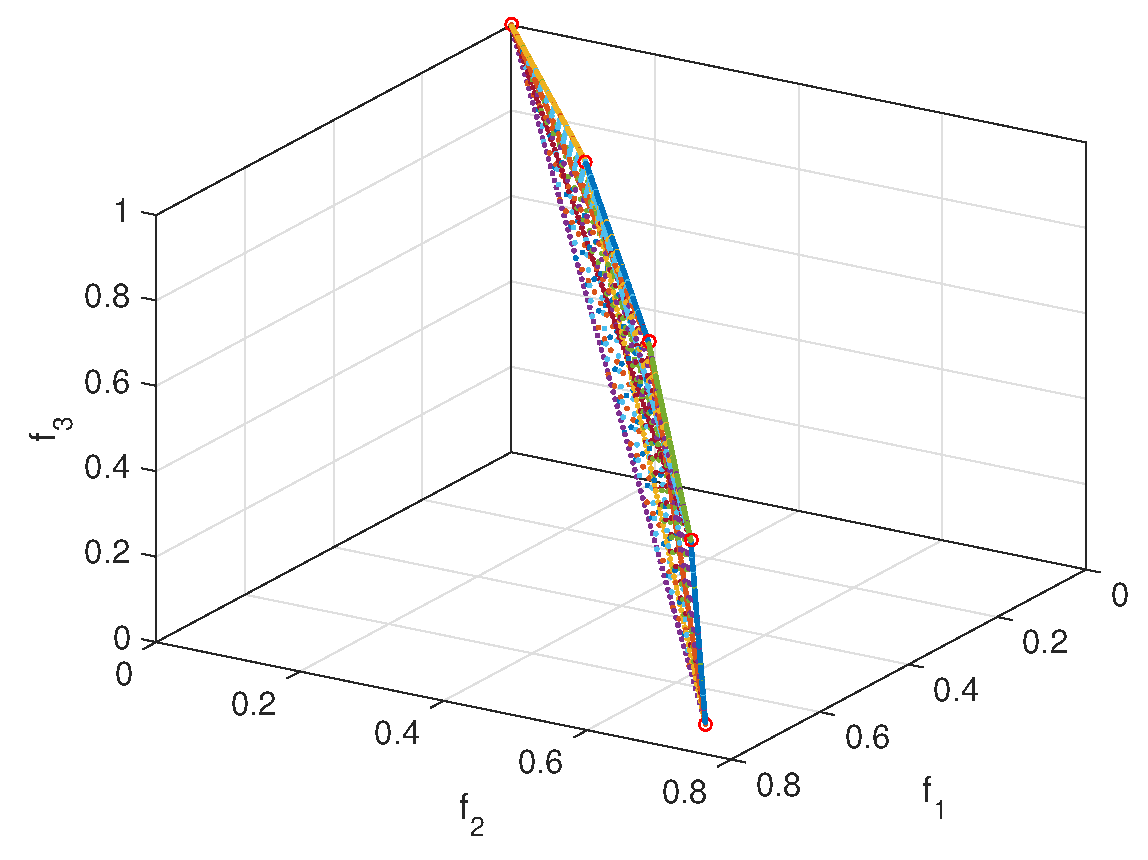
\includegraphics[width=.30\linewidth]{dtlz5_polytopeinit.eps}}
	\subfigure[]{\label{fig:dtlz5_approx}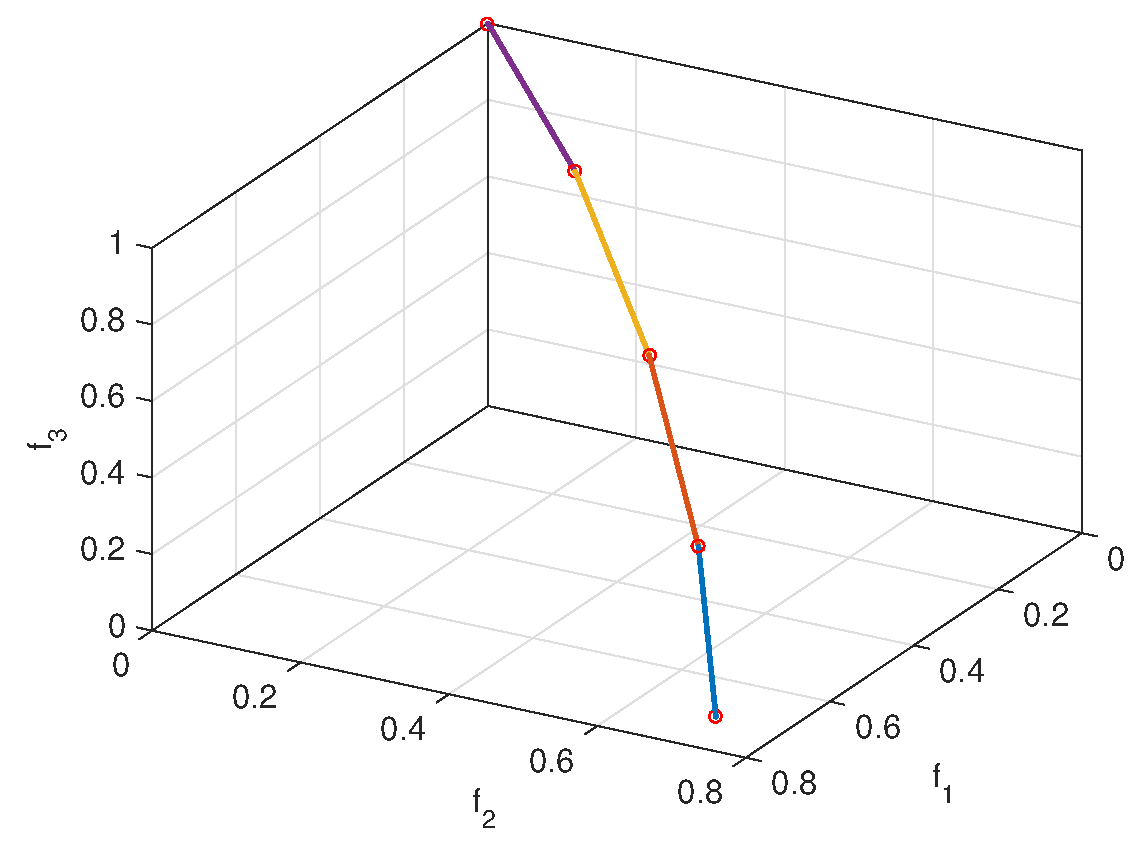
\includegraphics[width=.30\linewidth]{dtlz5_Approx.eps}}
	\subfigure[]{\label{fig:dtlz5_all}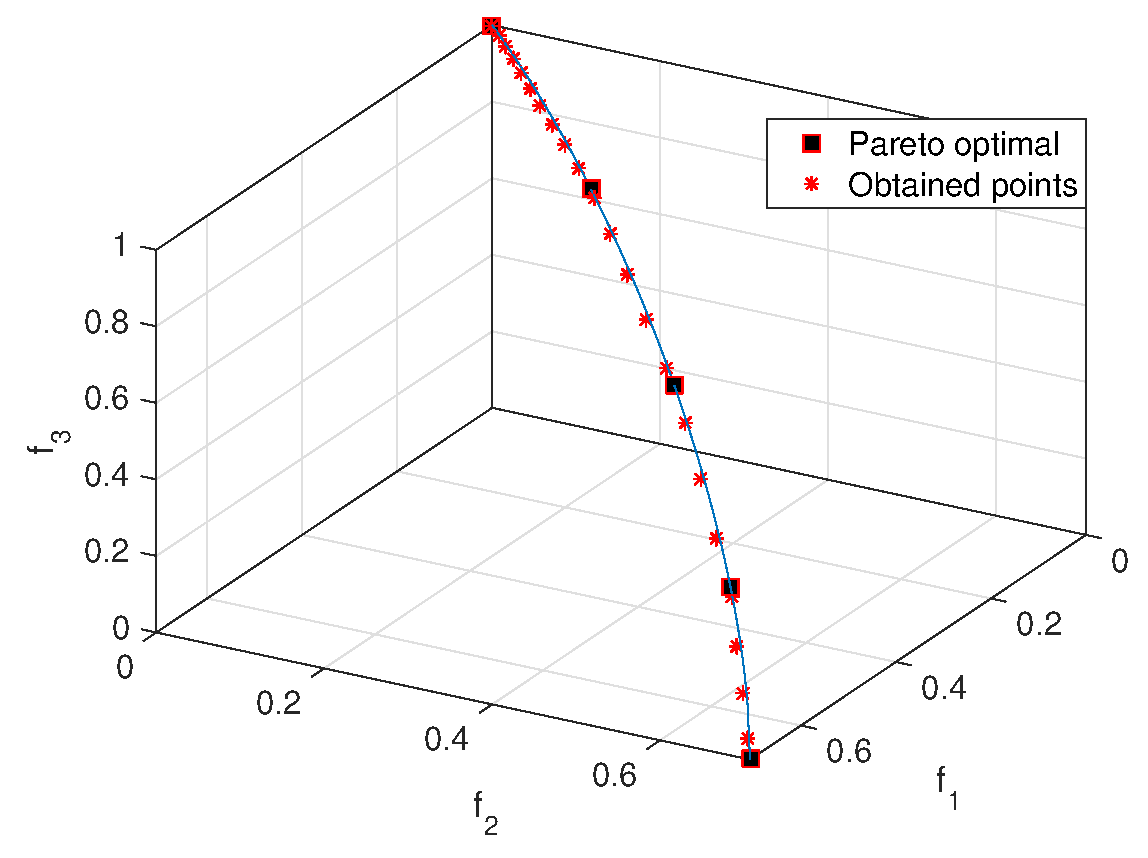
\includegraphics[width=.30\linewidth]{dtlz5_allpoint_990.eps}}
	\caption{DTLZ5: (a) Set of initial {\color{blue}simplexes} (b) Survived {\color{blue}simplexes} (c) Interpolated outcomes}
	\label{fig:dtlz5_true_approx}
\end{figure*}

The next problem~(three objective DTLZ7) involves an additional degree of challenge since the Pareto front consists of a curve~(line) and a surface~\cite{deb2002scalable}. The DM is provided with $12$ Pareto optimal outcomes. The results are presented in Figure~\ref{fig:dtlz7_true_approx}. There are several directions with multiple intersection resulting in $83$ unique interpolated outcomes and $82$unique reference directions are associated with interpolated outcome. 

\begin{figure*}[!ht]
	\centering
	\subfigure[]{\label{fig:dtlz7_init}\includegraphics[width=.30\linewidth]{dtlz7_polytopeinit.eps}}
	\subfigure[]{\label{fig:dtlz7_approx}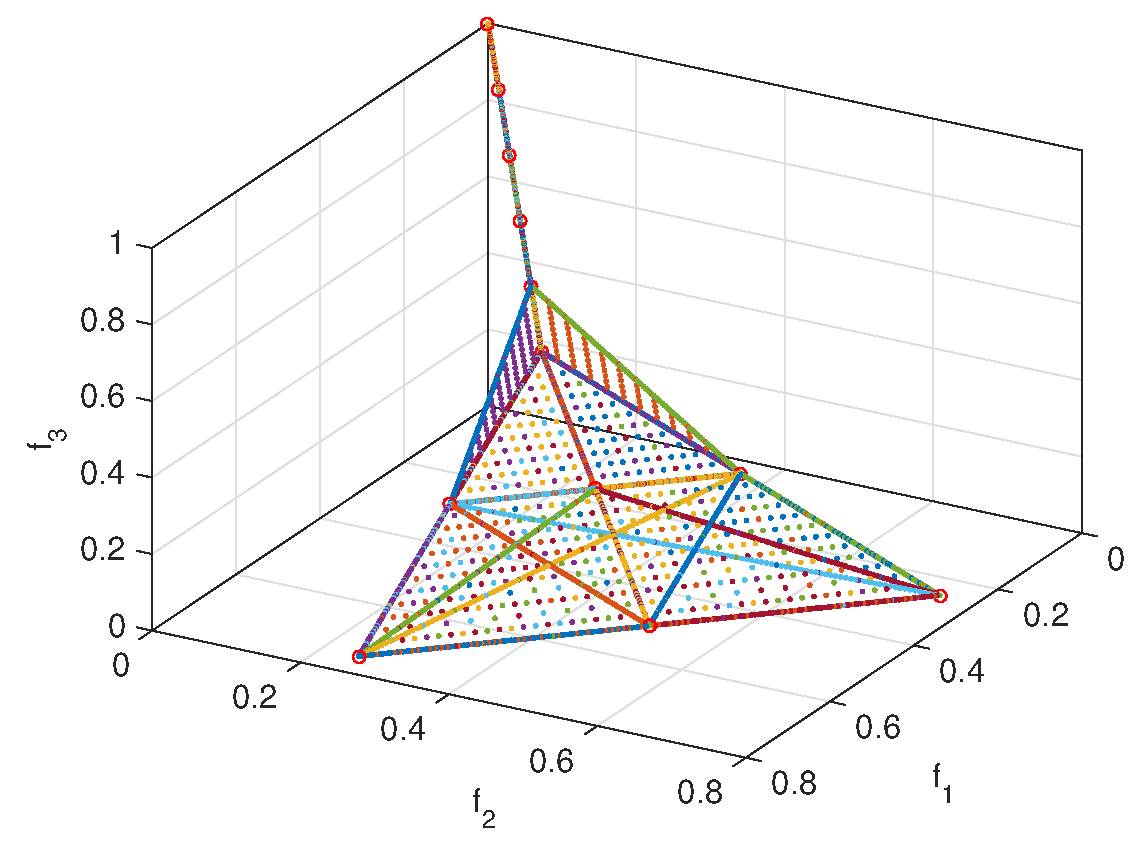
\includegraphics[width=.30\linewidth]{dtlz7_Approx.eps}}
	\subfigure[]{\label{fig:dtlz7_all}\includegraphics[width=.30\linewidth]{dtlz7_allpoint_300.eps}}
	\caption{DTLZ7: (a) Set of initial {\color{blue}simplexes} (b) Survived {\color{blue}simplexes} (c) Interpolated outcomes}
	\label{fig:dtlz7_true_approx}
\end{figure*}

The next problem represents yet another type of challenge, a mixed~(convex+concave) front. The $PF$ of the problem~(referred to here as hourglass) is synthetically constructed by concatenating two sets~($S_1$ and $S_2$) obtained using Equation~\ref{eqn:Hourglass}.

The DM is initially presented $55$ Pareto optimal outcomes. The interpolated outcomes with the theoretical Pareto front (in light blue background) and the corresponding metrics are shown in Figure~\ref{fig:mixed_dtlz2_true_approx}. Again for this problem, there are only $99$ directions are associated with an interpolated outcome~($99$ out of $300$). There are also reference directions with multiple interpolated outcomes as visible from Figure~\ref{fig:mixed_dtlz2_true_approx}.

\begin{equation}\small
\begin{aligned}
&\hspace{0em}\text{Input:}\quad\text{spacing}\; s, M = 3,\\
&\hspace{0em}\text{Generate set $W$ with}\quad N = {M+s-1\choose s}\; \\
&\hspace{0em}\text{(using systematic sampling)}\;,\\
&\hspace{0em}{P_1}_{i,j} = \frac{W_{i,j}}{\sqrt{\sum_{j = 1}^M} {W_{i,j}}^2},\;\forall\; i = 1,\dots, N \;\&\; j = 1,\dots,M, \\
&\hspace{0em}{S_1}_{i,j} = {P_1}_{i,j} + 1,\; \forall i = 1,\dots,N\; \&\;j = 1,\dots,M-1,\\ 
&\hspace{0em}{P_2}_{i,j} = 1 - {P_1}_{i,j},\\
&\hspace{0em}{S_2}_{i,j} = {P_2}_{i,j} + 1,\; \forall i = 1,\dots,N\; \&\;j = M,\\
&\hspace{0em}PF = S_1 \cup S_2
\label{eqn:Hourglass}
\end{aligned}
\end{equation}

\begin{figure*}[!ht]
	\centering
	\subfigure[]{\label{fig:mixed_dtlz2_init}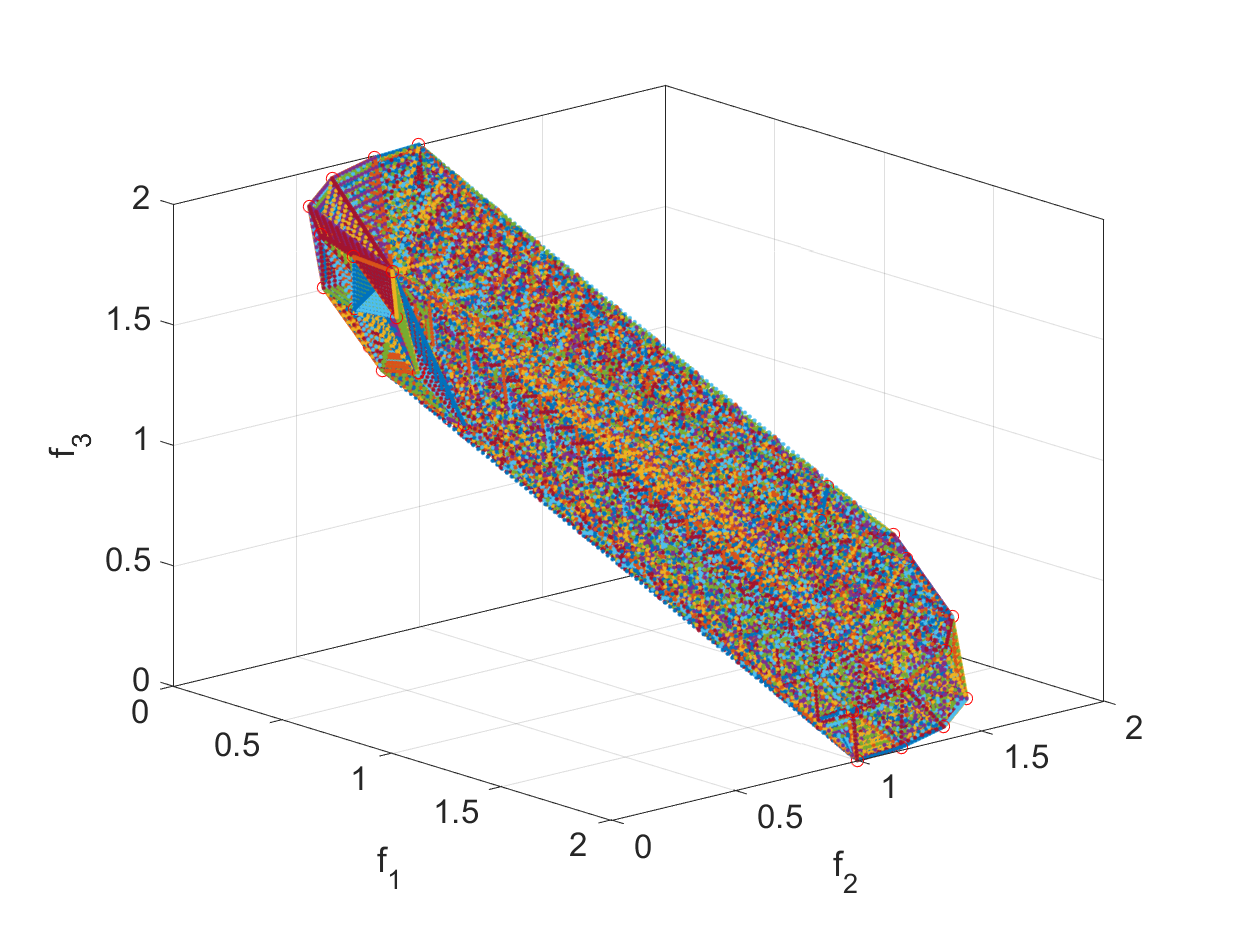
\includegraphics[width=.30\linewidth]{mixed_dtlz2_polytopeinit.eps}}
	\subfigure[]{\label{fig:mixed_dtlz2_approx}\includegraphics[width=.30\linewidth]{mixed_dtlz2_Approx.eps}}
	\subfigure[]{\label{fig:mixed_dtlz2_all}\includegraphics[width=.30\linewidth]{mixed_dtlz2_allpoint_300.eps}}
	\caption{Hourglass: (a) Set of initial {\color{blue}simplexes} (b) Survived {\color{blue}simplexes} (c) Interpolated outcomes}
	\label{fig:mixed_dtlz2_true_approx}
\end{figure*}

\subsection{Front with a void}
While in the above examples we highlighted the performance of the approach across a range of $PF$'s, we now highlight an important limitation of interpolation using just Pareto optimal outcomes. The three objective DTLZ2 problem is modified to have a void in its $PF$ at the center. The details of the construction of the $PF$ is presented in Equation~\ref{eqn:dtlz2c1}.

\begin{equation}\small
\begin{aligned}
\underset{\textbf{x}}{\operatorname{Minimize}}& \\
& \hspace{-1.5em}f_1(\textbf{x}) = (1+C(\textbf{x}))cos(\pi\frac{x_1}{2})cos(\pi\frac{x_2}{2}) \\
& \hspace{-1.5em}f_2(\textbf{x}) = (1+C(\textbf{x}))cos(\pi\frac{x_1}{2})sin(\pi\frac{x_2}{2}) \\ 
& \hspace{-1.5em}f_3(\textbf{x}) = (1+C(\textbf{x}))sin(\pi\frac{x_1}{2}) \\
\text{subject to}&\\
& \hspace{-1.5em}g(\textbf{x}) = 0.4 - rad \le 0 \\
& \hspace{-1.5em}0 \le x_1, x_2, x_3 \le 1,\\ 
& \hspace{-1.5em}C(\textbf{x}) = (x_3 - 0.5)^2,\\
& \hspace{-1.5em}rad = \text{perpendicular distance from a point}\\ 
& \hspace{-1.5em}\left[f_1, f_2, f_3\right] \text{to the line joining} \left[0, 0, 0\right] \text{and} \left[1, 1, 1\right]
\label{eqn:dtlz2c1}
\end{aligned}
\end{equation} 

The interpolated outcomes are presented in Figure~\ref{fig:dtlz2c1_approx}. The theoretical Pareto front (in light blue background) and the reduced set of interpolated outcomes are presented in Figure~\ref{fig:dtlz2c1_all}. One can clearly observe that the proposed approach cannot detect the presence of the hole although the given set of $28$ Pareto optimal outcomes did not have any solutions within the hole. The positive and negative dominance measure for the obtained outcomes inside the void will be higher than the outcomes elsewhere. Nearest neighbor distance metric as depicted in Figure~\ref{fig:dtlz2c1_mindist} suggests that outcomes within the hole are in general far from the given set of Pareto optimal outcomes. Thus one should exercise caution to select such outcomes as reference points. The key utility of the proposed metrics is in identifying such cases. Total number of interpolated outcomes for this problem is $1727$ along $300$ unique set of reference directions. 

\begin{figure*}[!ht]
	\centering
	\subfigure[]{\label{fig:dtlz2c1_init}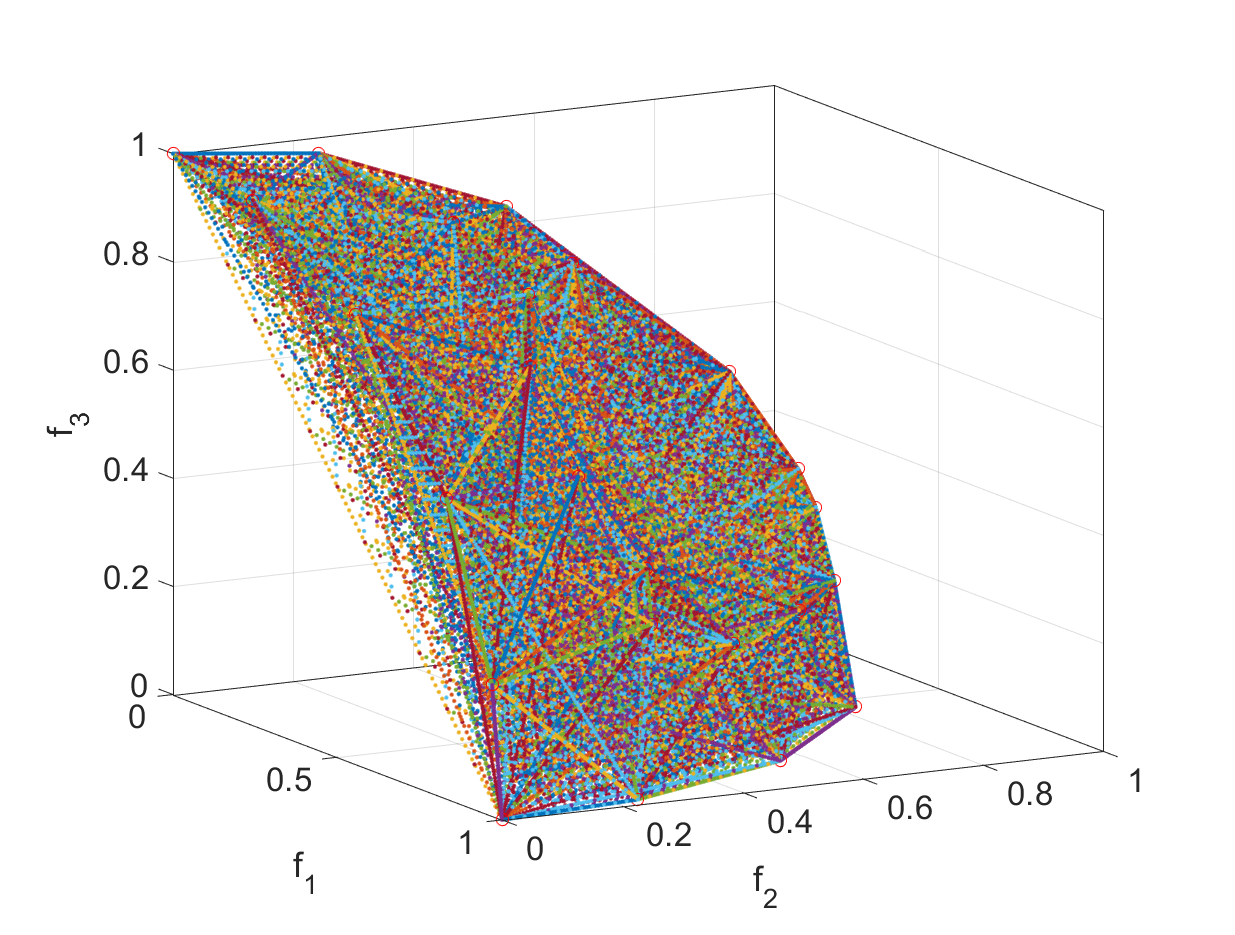
\includegraphics[width=.30\linewidth]{dtlz2c1_polytopeinit.eps}}
	\subfigure[]{\label{fig:dtlz2c1_approx}\includegraphics[width=.30\linewidth]{dtlz2c1_Approx.eps}}
	\subfigure[]{\label{fig:dtlz2c1_all}\includegraphics[width=.30\linewidth]{dtlz2c1_allpoint_300.eps}}\\
	\subfigure[]{\label{fig:dtlz2c1_eps}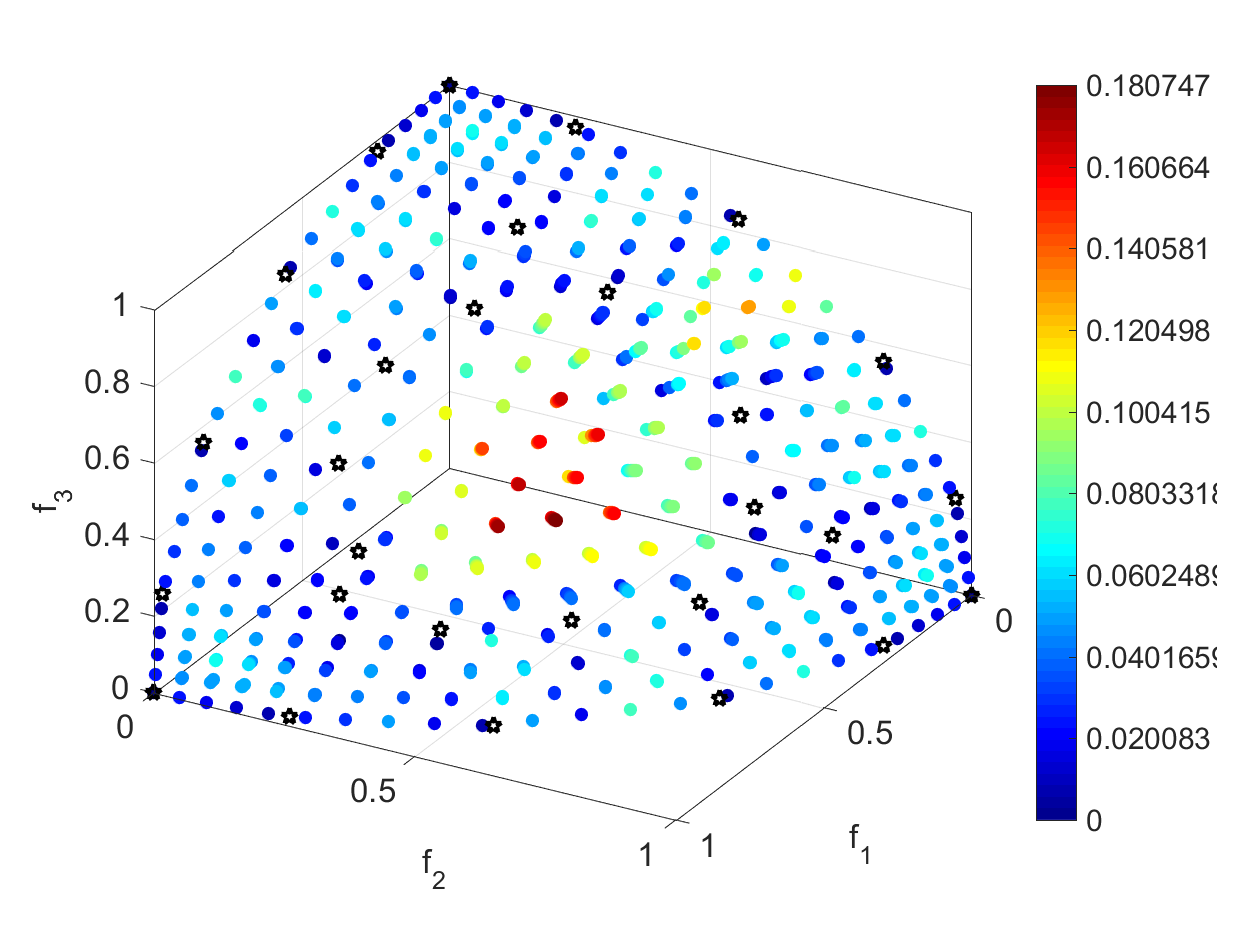
\includegraphics[width=.30\linewidth]{dtlz2c1_epsdom.eps}}
	\subfigure[]{\label{fig:dtlz2c1_reveps}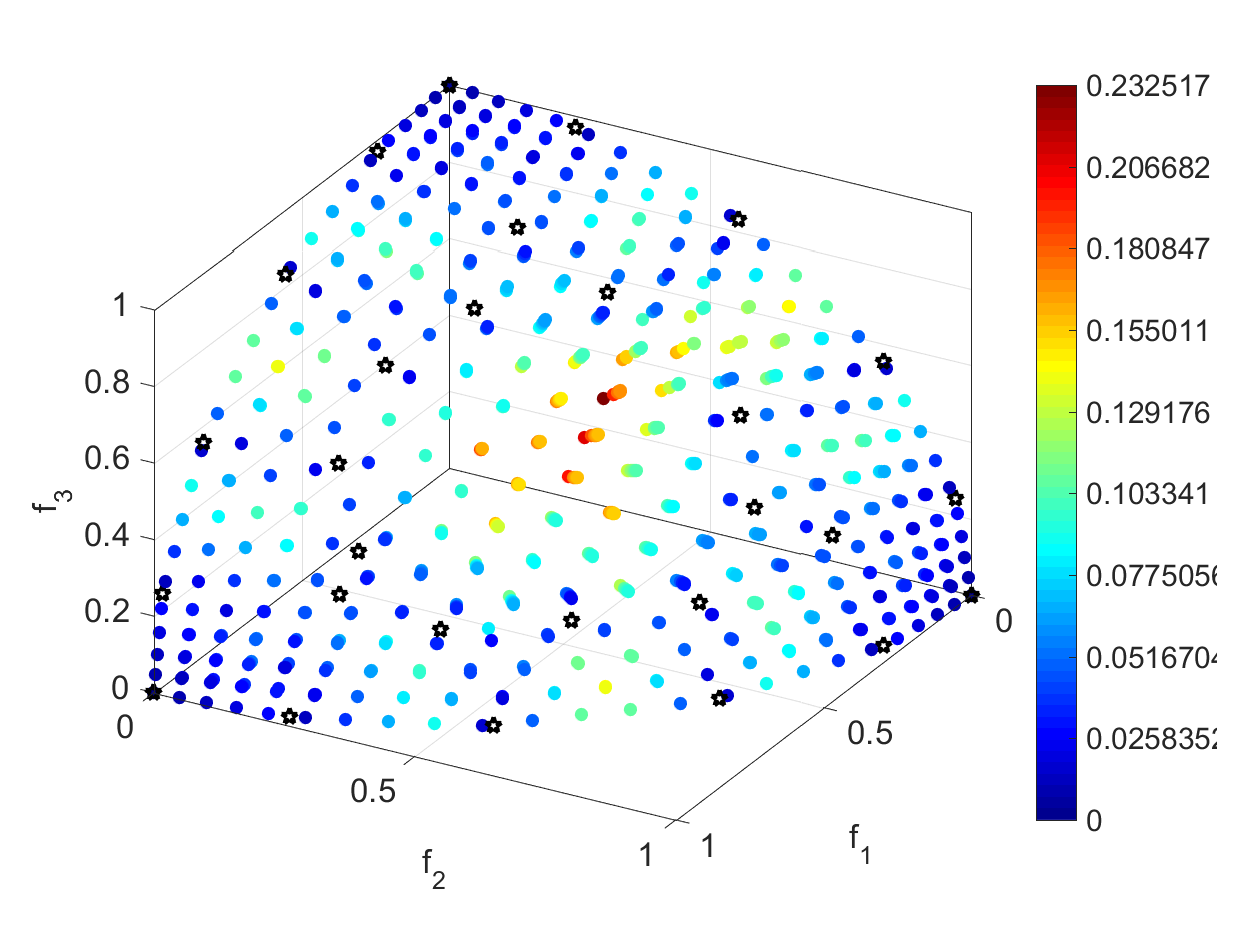
\includegraphics[width=.30\linewidth]{dtlz2c1_epsrevdom.eps}}
	\subfigure[]{\label{fig:dtlz2c1_mindist}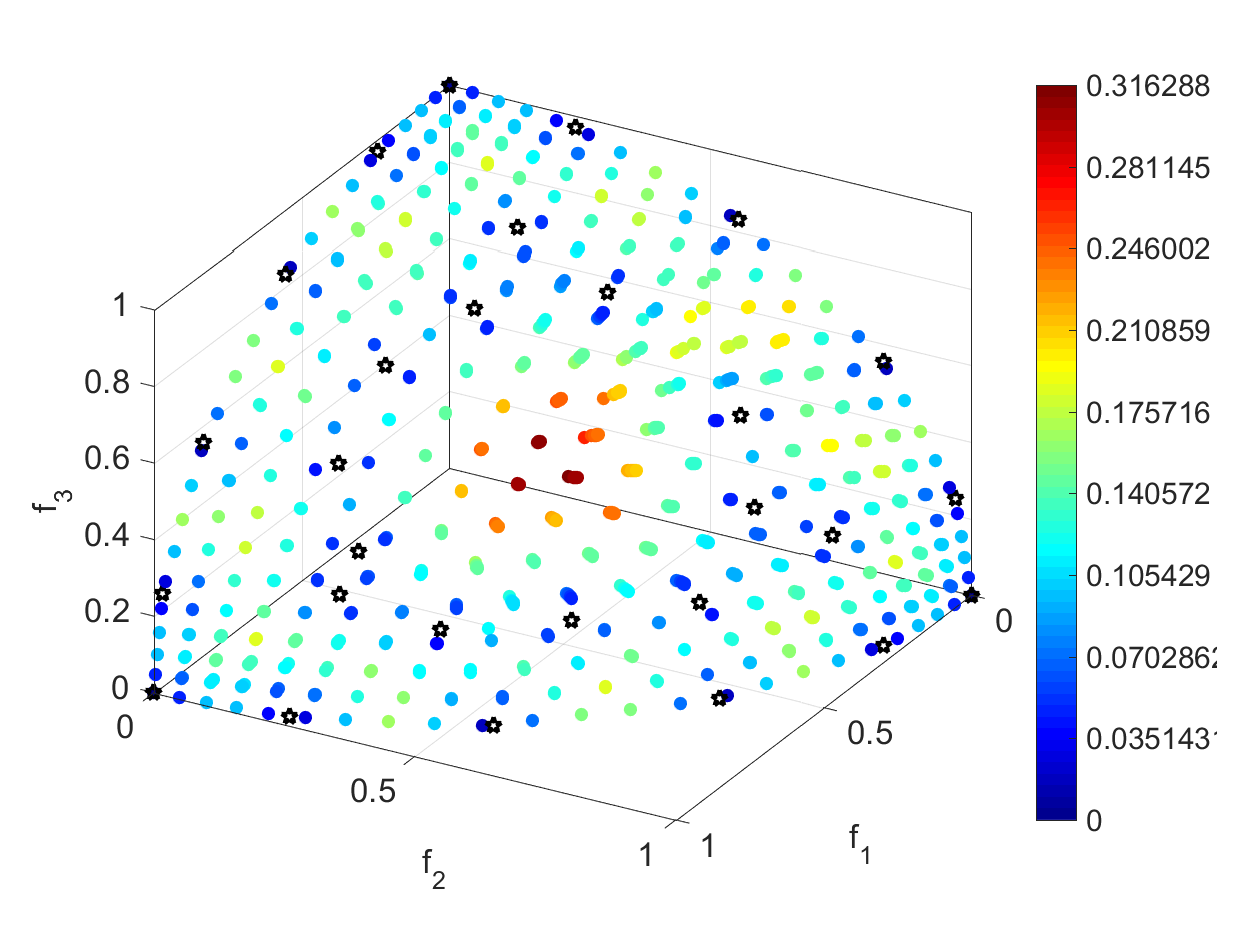
\includegraphics[width=.30\linewidth]{dtlz2c1_mindist_300.eps}}
	\caption{DTLZ2-mod: (a) Set of initial {\color{blue}simplexes} (b) Survived {\color{blue}simplexes} (c) Interpolated outcomes (d) Negative dominance measure (e) Positive dominance measure (f) Nearest neighbor distance}
	\label{fig:dtlz2c1_true_approx}
\end{figure*}

\subsection{Forest management}
In the above set of test problems, the initial set of Pareto optimal outcomes were uniformly distributed. We now observe the performance of the proposed approach using $20$ non-uniform Pareto optimal outcomes for a practical problem. The forest management problem is taken from \cite{eyvindson2013towards}. The problem considers three objectives: net income, total standing wood volume and old growth at the end of ten years period. The initial and survived simplex set, interpolated outcomes and corresponding metrics are presented in Figure~\ref{fig:forest_true_approx}. One can observe that there are only $120$ unique ($120$ out of $300$) directions having at least one intersection. The presence of $109$ surviving $2-${\color{blue}simplexes} listed in Table~\ref{tab:probstat} suggest that the $PF$ is non-degenerate.

\begin{figure*}[!ht]
	\centering
	\subfigure[]{\label{fig:forest_init}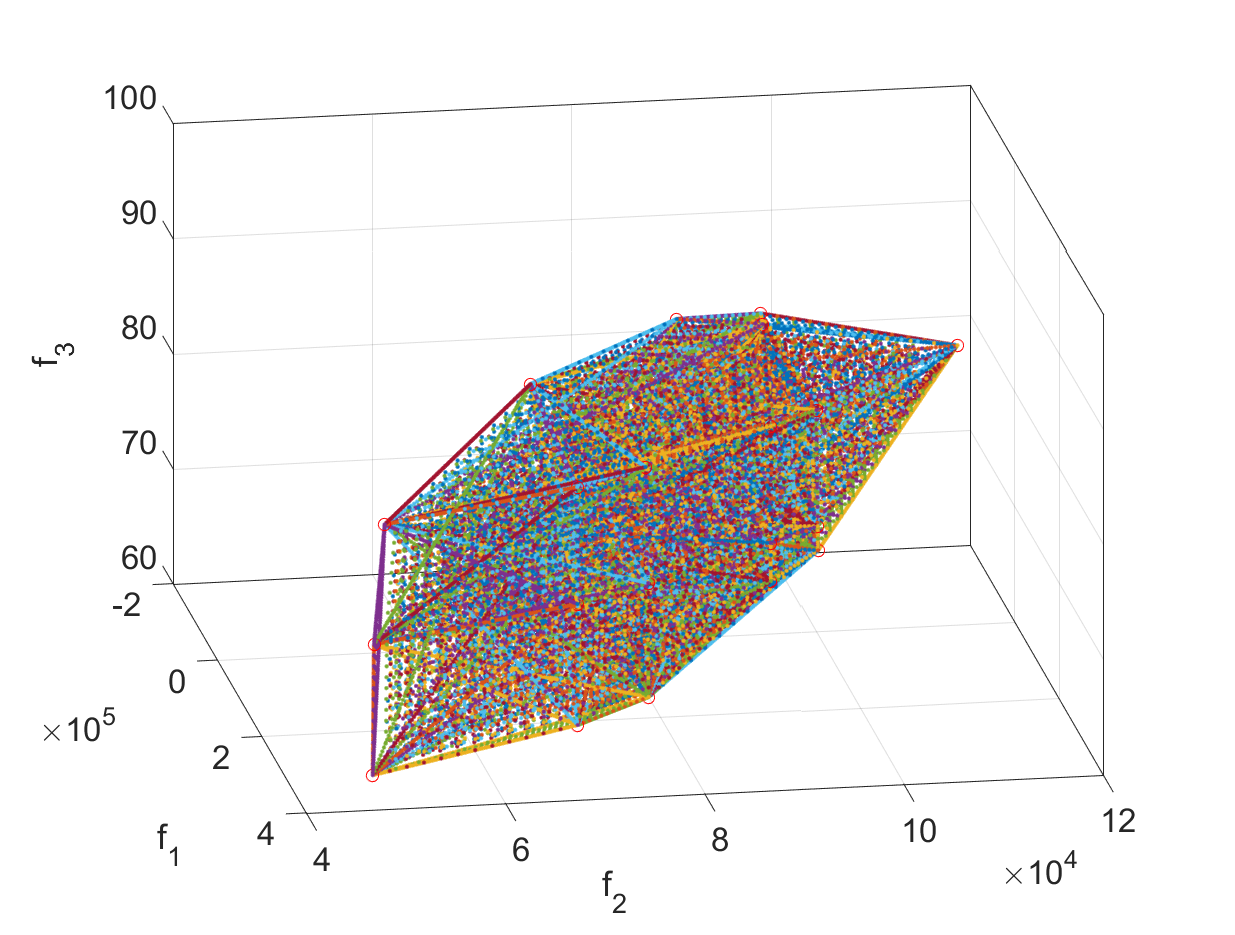
\includegraphics[width=.30\linewidth]{forest_polytopeinit.eps}}
	\subfigure[]{\label{fig:forest_approx}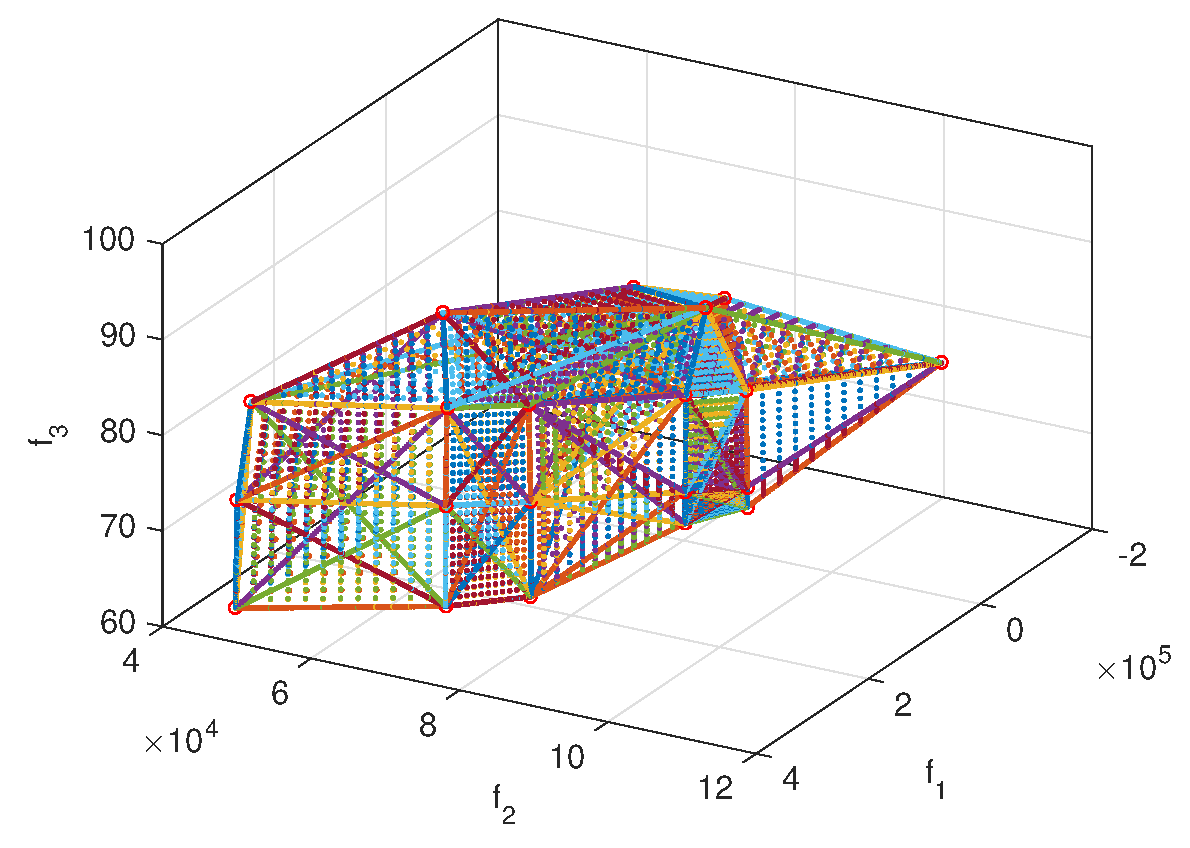
\includegraphics[width=.30\linewidth]{forest_Approx.eps}}
	\subfigure[]{\label{fig:forest_all}\includegraphics[width=.30\linewidth]{forest_allpoint_300.eps}}\\
	\subfigure[]{\label{fig:forest_eps}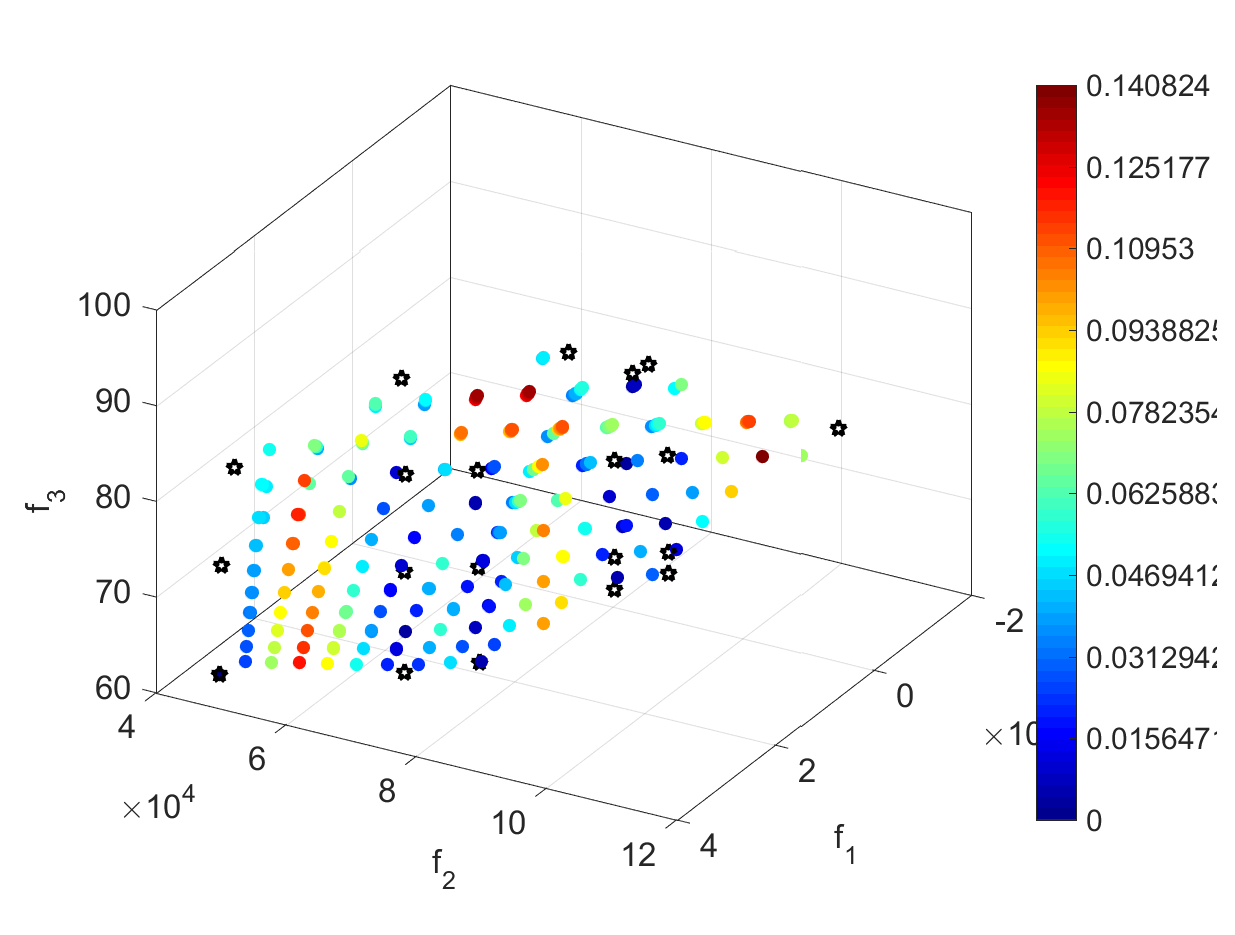
\includegraphics[width=.30\linewidth]{forest_epsdom.eps}}
	\subfigure[]{\label{fig:forest_reveps}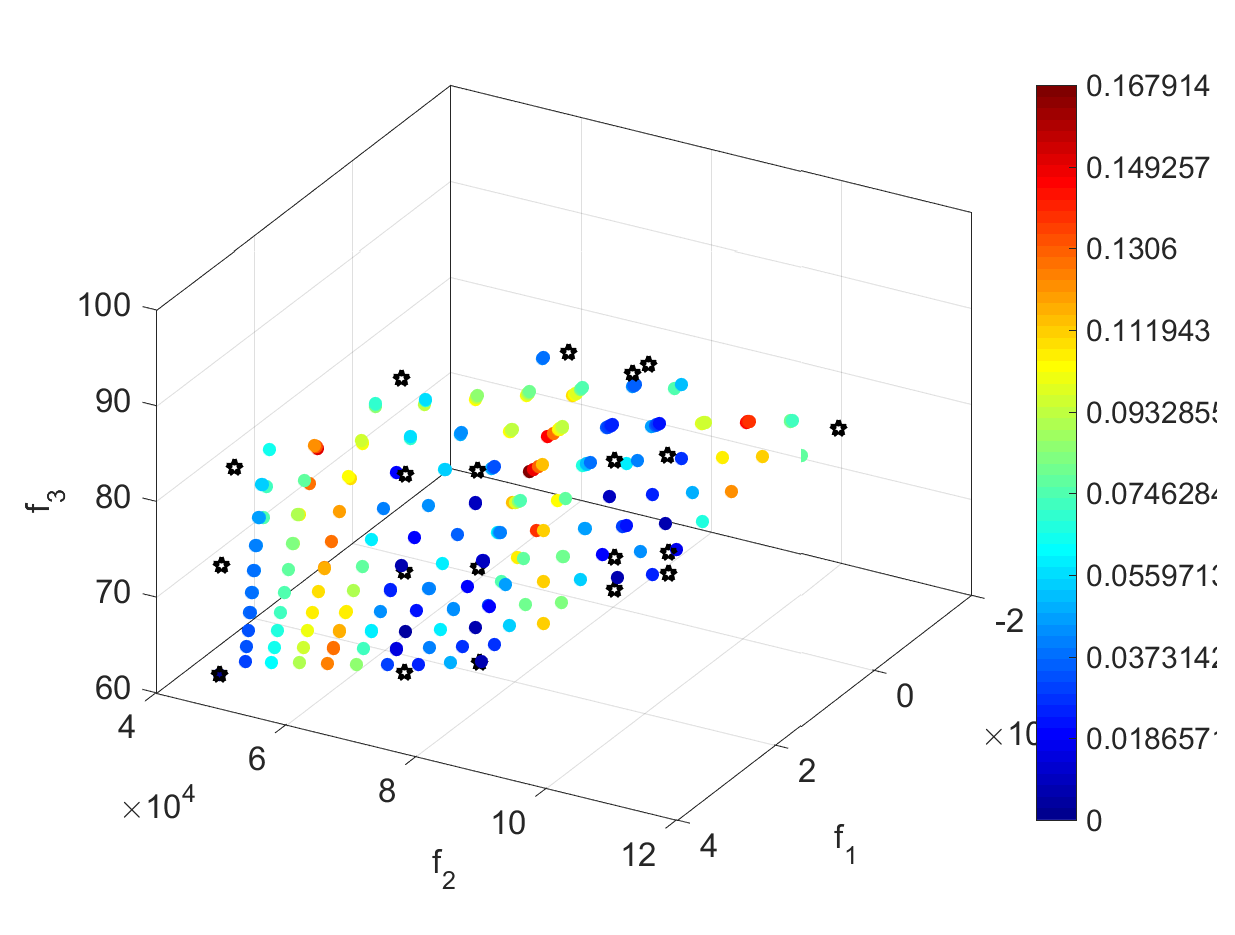
\includegraphics[width=.30\linewidth]{forest_epsrevdom.eps}}
	\subfigure[]{\label{fig:forest_mindist}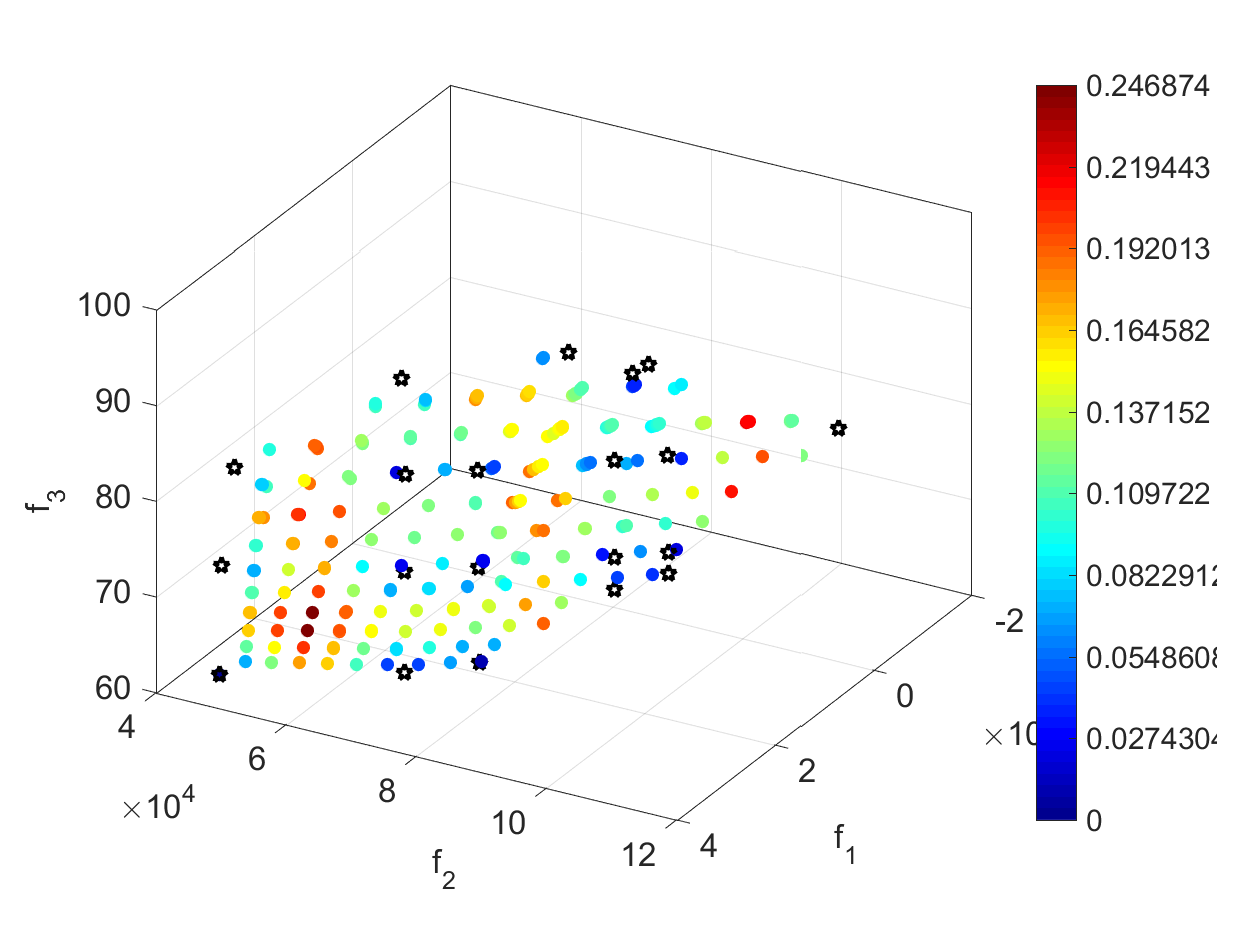
\includegraphics[width=.30\linewidth]{forest_mindist_300.eps}}
	\caption{Forest management: (a) Set of initial {\color{blue}simplexes} (b) Survived {\color{blue}simplexes} (c) Interpolated outcomes (d) Negative dominance measure (e) Positive dominance measure (f) Nearest neighbor distance}
	\label{fig:forest_true_approx}
\end{figure*}

\subsection{Heat exchanger design}
This practical optimization problem relates to design of a heat exchanger, taken from  \cite{hartikainen2010computationally}. There are three objectives that are to be minimized: number of heat exchanger units, total heat exchanger surface area and hot utility consumption. The total number of unique Pareto optimal outcomes presented to the DM is $8$ ~($9$ in ~\cite{hartikainen2010computationally} as a duplicate point was listed). The given Pareto optimal outcomes are listed in Table~\ref{probstatheat1}. The interpolated outcomes and the corresponding metrics are presented in Figure~\ref{fig:heat_exchanger_true_approx}.

\begin{figure*}[!ht]
	\centering
	\subfigure[]{\label{fig:heat_exchanger_init}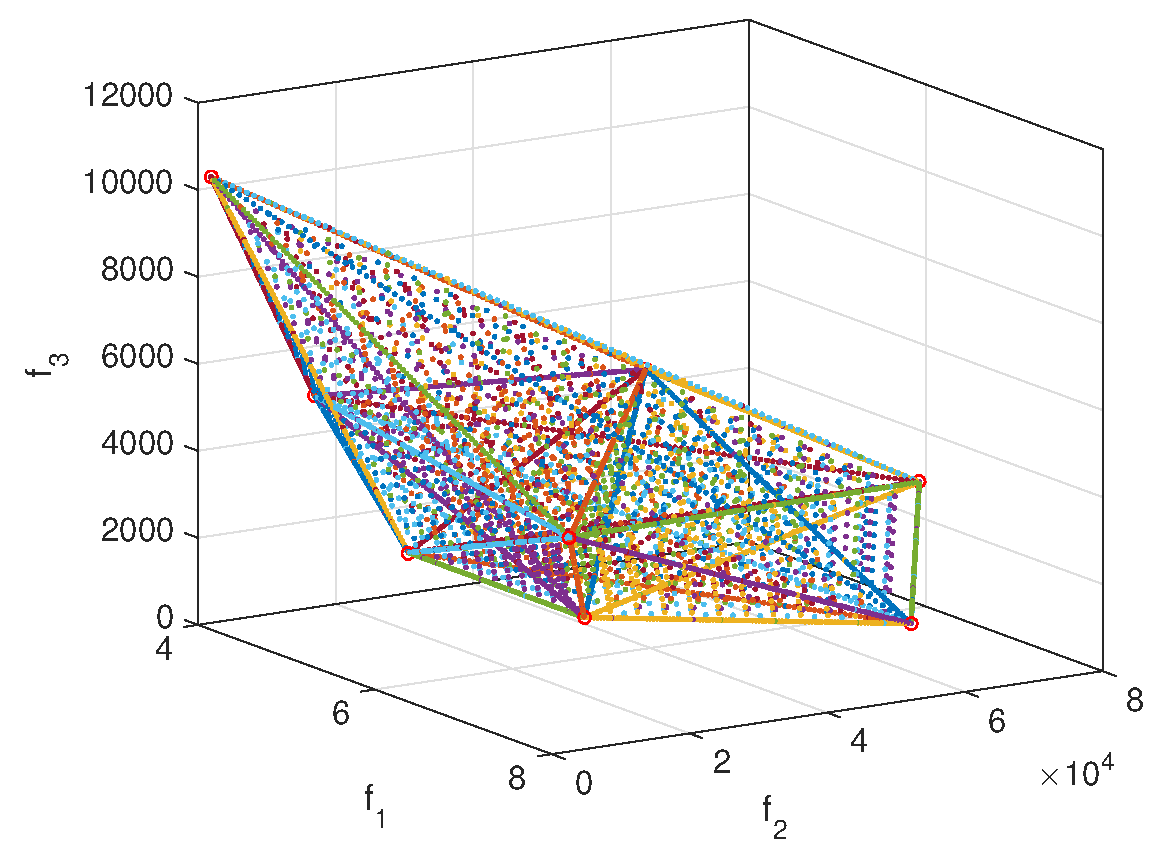
\includegraphics[width=.30\linewidth]{heat_exchanger_polytopeinit.eps}}
	\subfigure[]{\label{fig:heat_exchanger_approx}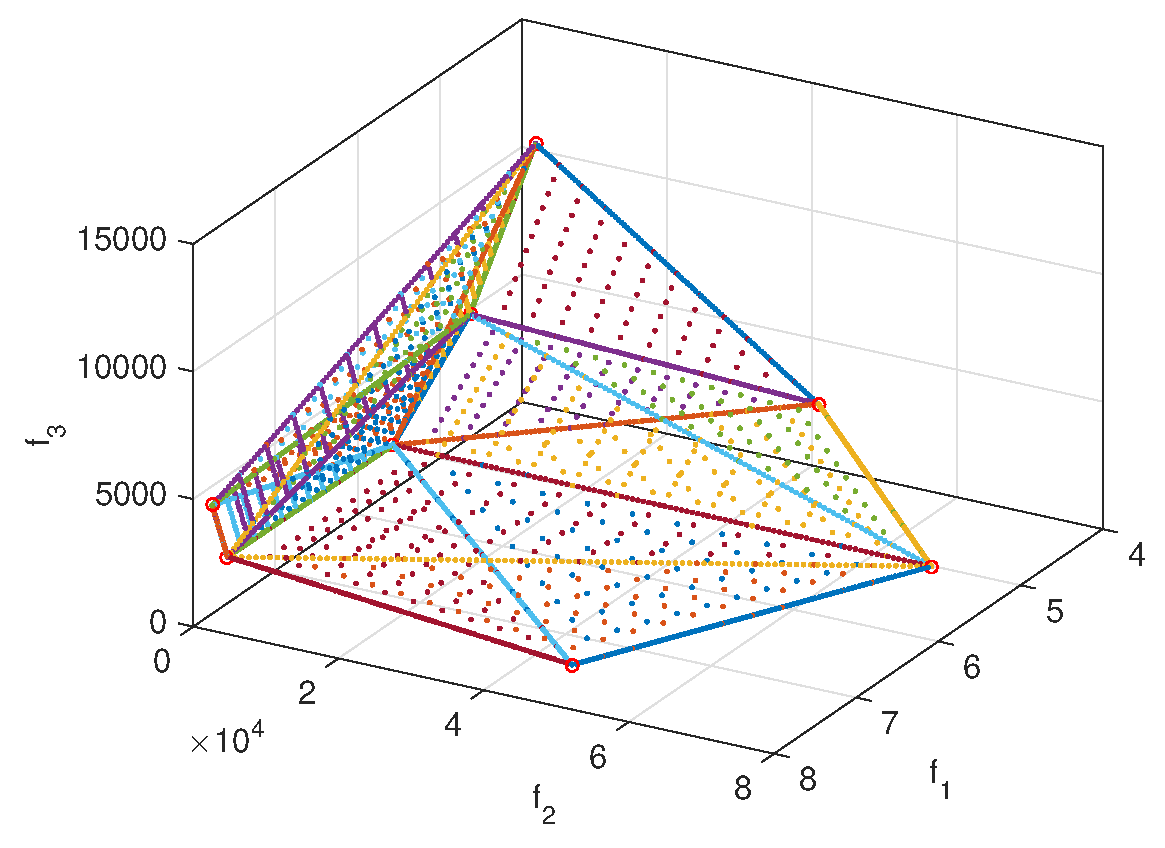
\includegraphics[width=.30\linewidth]{heat_exchanger_Approx.eps}}
	\subfigure[]{\label{fig:heat_exchanger_all}\includegraphics[width=.30\linewidth]{heat_exchanger_allpoint_300.eps}}\\
	\subfigure[]{\label{fig:heat_exchanger_eps}\includegraphics[width=.30\linewidth]{heat_exchanger_epsdom.eps}}
	\subfigure[]{\label{fig:heat_exchanger_reveps}\includegraphics[width=.30\linewidth]{heat_exchanger_epsrevdom.eps}}
	\subfigure[]{\label{fig:heat_exchanger_mindist}\includegraphics[width=.30\linewidth]{heat_exchanger_mindist_300.eps}}
	\caption{Heat exchanger: (a) Set of initial {\color{blue}simplexes} (b) Survived {\color{blue}simplexes} (c) Interpolated outcomes (d) Negative dominance measure (e) Positive dominance measure (f) Nearest neighbor distance}
	\label{fig:heat_exchanger_true_approx}
\end{figure*}

One can observe that there are no voids~(missing faces) in our interpolation~(Figure~\ref{fig:heat_exchanger_pli}) which is in contrast with the results reported in~\cite{hartikainen2010computationally} using PAINT. There are $47$ {\color{blue}simplexes} that survive. The details of the {\color{blue}simplexes} are listed in Table~\ref{tab:probstatheat2}.  We highlight that the inherently non-dominated interpolated outcomes delivered by PAINT~\cite{hartikainen2010computationally} did not have several $1$ and $2-${\color{blue}simplexes}~($1-${\color{blue}simplexes}: P21, P25, P26, P27, P28; $2-${\color{blue}simplexes}: P30, P31, P34, P35, P38, P41, P42, P43, P44, P45, P46, and P47). Once again for this problem, $156$ unique reference directions had interpolated outcome~($156$ out of $300$) and there were multiple intersections along several directions as visible form Table~\ref{tab:probstat}). 


\begin{table}[h]\scriptsize
	\centering
	\caption{Starting set of Pareto optimal outcomes for the heat exchanger problem}
	\label{probstatheat1}
	\tabcolsep=0.11cm
	%\begin{tabular}{llll}
	\begin{tabular}{p{1cm}p{1.2cm}p{2.5cm}p{2.5cm}}
		\specialrule{.1em}{.1em}{.1em} 
		{\bf Point} & {\bf Number of heat exchanger units} & {\bf Total heat exchanger surface area} & {\bf Hot utility consumption} \\ \hline
		v1          & 4                                    & 1897                                    & 10250                         \\ \hline
		v2          & 8                                    & 52175                                   & 1755                          \\ \hline
		v3          & 5                                    & 52175                                   & 5371                          \\ \hline
		v4          & 6                                    & 4913                                    & 3028                          \\ \hline
		v5          & 8                                    & 4734                                    & 3028                          \\ \hline
		v6          & 8                                    & 2608                                    & 4920                          \\ \hline
		v7          & 6                                    & 79064                                   & 2882                          \\ \hline
		v8          & 5                                    & 4153                                    & 5902                          \\
		\specialrule{.1em}{.1em}{.1em}
	\end{tabular}
\end{table}
%\vspace{-20em}
\begin{table}[!ht]\scriptsize
	\centering
	\caption{Surviving {\color{blue}simplexes} for heat exchanger problem}
	\label{tab:probstatheat2}
	\tabcolsep=0.11cm
	\begin{tabular}{llllll}
		\specialrule{.1em}{.1em}{.1em} 
		{\bf {\color{blue}Simplex}} & {\bf Vertices} & {\bf {\color{blue}Simplex}} & {\bf Vertices} & {\bf {\color{blue}Simplex}} & {\bf Vertices} \\ \hline
		P1             & v1             & P17            & v3 v4          & P33            & v1 v5 v6       \\ \hline
		P2             & v2             & P18            & v3 v7          & P34            & v1 v5 v8       \\ \hline
		P3             & v3             & P19            & v3 v8          & P35            & v1 v6 v8       \\ \hline
		P4             & v4             & P20            & v4 v5          & P36            & v2 v4 v5       \\ \hline
		P5             & v5             & P21            & v4 v6          & P37            & v2 v4 v7       \\ \hline
		P6             & v6             & P22            & v4 v7          & P38            & v2 v5 v7       \\ \hline
		P7             & v7             & P23            & v4 v8          & P39            & v3 v4 v7       \\ \hline
		P8             & v8             & P24            & v5 v6          & P40            & v3 v4 v8       \\ \hline
		P9             & v1 v3          & P25            & v5 v7          & P41            & v3 v7 v8       \\ \hline
		P10            & v1 v4          & P26            & v5 v8          & P42            & v4 v5 v6       \\ \hline
		P11            & v1 v5          & P27            & v6 v8          & P43            & v4 v5 v7       \\ \hline
		P12            & v1 v6          & P28            & v7 v8          & P44            & v4 v5 v8       \\ \hline
		P13            & v1 v8          & P29            & v1 v3 v8       & P45            & v4 v6 v8       \\ \hline
		P14            & v2 v4          & P30            & v1 v4 v5       & P46            & v4 v7 v8       \\ \hline
		P15            & v2 v5          & P31            & v1 v4 v6       & P47            & v5 v6 v8       \\ \hline
		P16            & v2 v7          & P32            & v1 v4 v8       &                &                \\ \specialrule{.1em}{.1em}{.1em}
	\end{tabular}
\end{table}

\section{Summary and Future work}
\label{sec:sum}

Constructing piecewise linear interpolations from a given set of Pareto outcomes is an interesting problem, with significant utility in multi-attribute decision making. In the context of interactive multi/many objective optimization and problems involving expensive analysis~(computational or physical experiments), the number of available solutions and their corresponding outcomes may be only a handful. Identification of regions of interest from such a sparse set of Pareto optimal outcomes is known to be challenging. The proposed method builds a piecewise linear interpolation from the given Pareto outcome set to assist the decision maker in identifying regions of interest for such class of the problems. The specific contributions of the work in light of existing interpolation approaches are summarized below:

\begin{enumerate}
	\item The limitations of the-state-of-the-art PAreto INTerpolation~(PAINT) approach {\color{blue}were highlighted, in which the use of Delaunay triangulation and strict enforcement of inherent non-dominance allows for existence of only one~(out of potentially many) possible interpolation~(simplex set) and may in some cases lead to undesirable voids/discontinuities in the interpolation. 
		\item A piecewise linear interpolation method is proposed, which aims to deliver a comprehensive set of all possible linear valid interpolations which are non-dominated with respect to the given Pareto optimal outcomes; instead of its subset generated by existing approaches. The computational complexity of the approach is shown to be advantageous~(for high objectives) which is further improved by its ability to be executed in a parallel mode. 
		\item A number of contemporary algorithms use systematic sampling using NBI. In-line with this practice, the proposed approach further delivers a set of uniformly distributed set of interpolated outcomes~(from the comprehensive interpolation obtained above as a collection of simplexes). These could be presented to a decision maker as additional~(though approximated) alternatives to find regions of interest that could be explored further.  
		\item Two metrics, based on dominance and nearest neighbor distance were used to estimate the quality of the interpolated outcomes. Such information could further aid decision making, in a sense that the effort required in pursuing a true Pareto outcome in a particular region could be weighed against confidence established by the error measures of the interpolated outcomes in that region.
		\item The performance of the proposed technique was illustrated on several examples. These included convex,non-convex, mixed and degenerate sets of Pareto outcomes. Further, studies on two real life problems~(heat exchanger and forest management) were also presented. 
	}
\end{enumerate}

Several potential future directions could be pursued to extend the presented work. Development of means to detect voids in the Pareto outcome space remains a challenge and there are some interesting attempts in~\cite{hartikainen2014paint} towards solving it. For the case of linear fronts~(e.g. DTLZ1), redundancy could be avoided by detecting and removing overlapping linear {\color{blue}simplexes} to deliver a sufficient minimal set of surviving {\color{blue}simplexes}. While attempts to uncover relationships in the decision variable space is well studied, the problem of learning information for even a given Pareto outcome set in higher dimensions, especially using sparse points is another challenge which is less talked about. Further improvement in run-time of the presented algorithms can be achieved by limiting number of LP calls invoked to detect intersections between a reference direction and all surviving {\color{blue}simplexes}. Lastly, while this paper considered the initial set of solutions as Pareto optimal outcomes, methods to deal with a more generic case, i.e., when a DM is presented with a set of infeasible and feasible solutions and would want to identify regions of interest, could be another interesting direction to explore. 
 

